\documentclass[]{report}
\usepackage[top=25mm, bottom=25mm, left=25mm, right=25mm]{geometry}
\usepackage{amsmath, amsfonts, amssymb, amsthm, physics, graphicx, wrapfig}
\usepackage{hyperref}
\usepackage{cleveref}
\usepackage{xcolor}
\usepackage{moreverb}

\usepackage[backend = biber]{biblatex}
\addbibresource{/home/perezsalinas/Escritorio/Mibiblioteca.bib}

\newcommand{\sign}{\ensuremath{\operatorname{sign}}}
\newcommand{\alert}[1]{{\color{red} #1}}

\title{{\Huge \textbf{Course in (Quantum) Machine Learning} \\ 
}}
\author{{\huge Adrián Pérez-Salinas} \\ \newline
$
\langle aQa \rangle^L$: Applied Quantum Algorithms, Leiden University, The Netherlands}
\date{\large\today}
\begin{document}
\maketitle
\tableofcontents

\chapter{Introduction}\label{ch.introduction}

The discipline of machine learning comprises a large variety of algorithms and techniques with the objective of making a machine automatically understand the hidden relationships of a training data. Machine learning has witnessed in recent years an exponential increment in its capabilities and in the influence it has on society. Some of the most celebrated examples nowadays are generative models, exemplified by Chat-GPT or Dall-E, although there have been many other examples applied to hard problems, such as protein folding \cite{jumper2021highly}. 

Machine learning has enabled us to make use of the gigantic power of data to address problems that were considered intractable beforehand. 

\section{What is machine learning}\label{sec.what-is}

We can begin by describing what is machine learning from a technical perspective. The central elements of machine learning will be covered in the subsequent paragraphs. 

\paragraph{Machine learning model}

    A machine learning model is a program $f$ with an input $x$ and an output $f(x)$, performing an operation to be determined by data. The models $f$ are usually specified by an architecture and a set of tunable parameters $\theta$. This means that an architecture is capable of realizing a large family of models $\mathcal F = \{ f_\theta\}_\theta$, and we will need to adjust the parameters $\theta$ to find the optimal function. 

    Machine learning models can follow a large variety of architectures, to be specified later. Some architectures are more suited to some problems than other. For example, convolutional neural networks are highly convenient to deal with problems in which data is given in the form of images. Another examples are transformers, which have been extensively used in large language models. Multilayer fully connected neural networks have also been used with wide purposes. When training the parameters $\theta$, the learning model finds an optimal solution \textit{within} the architecture, but cannot outperform the architecture itself. 

\paragraph{Data}

    In machine learning models, data is given by the pairs $(x, y)$, where $x$ will be the data input into the model, and $y$ will be output from the model. In certain cases, this data is truncated to only $x$. This data will be generically referred to as $\mathcal D = \mathcal X \times \mathcal Y$. The structure of the data \textit{in principle} contains all information required to solve a particular problem. The goal of a machine learning algorithm is to infer from data the implicit function $f : \mathcal X \rightarrow \mathcal Y$, with the aim that we can predict the effect of this function on previously unseen data. 

    Data can be divided in several types of data, for instance training set, test set or validation set. Before delving into the differences of these kinds of data it is important to highlight some particularities of the framework. The data points $\mathcal D$ conform a distribution of points $(x,y)$ which is in many cases continuous. In other words, one cannot access to all data available in $\mathcal D$, but only sample from it. This gives rise to the concept of training/test data. 

    \textit{Training data} is the discrete subset of data $\mathcal T = \{ (x, y)\}, (x,y) \sim \mathcal D$ used to train a model. The goal of the model, in broad terms, is to design a function $f$ such that $f(x) \approx y(x)$ for all, or the majority, of data pairs $(x, y)$. 

    \textit{Test data} is another discrete subset $\mathcal C$ of the same form as $\mathcal T$, that is not used to train the machine learning model. However, the success of the model depends on the performance over $\mathcal C$. Would the model perform accurately on $\mathcal C$, the model is considered successful. In this scenario, the model will have \textit{learnt} the data, as opposed to \textit{memorizing} it. Hence, the model is capable of generalizing the acquired knowledge. 

    There exists also the \textit{validation set} $\mathcal V$, as a third dataset serving as a touchstone of machine learning model. The $\mathcal V$ is used to adjust the outcomes of a machine learning model after training. This step is not always necessary or used, but it is very common. 

\paragraph{Training} A fundamental step of all machine learning algorithms is the optimization of the parameters, or training the model. To perform training, one needs a) a training dataset and b) a training algorithm. The goal of the training is to minimize some cost function that quantifies how accurately is the algorithm predicting the outcomes of a data set. 

The first ingredient is the loss function $\mathcal L(\theta)$, which can be computed with respect to different datasets, namely
\begin{equation}
    \mathcal L_{\mathcal D}(\theta), \qquad \mathcal L_{\mathcal T}(\theta), \qquad \mathcal L_{\mathcal C}(\theta)
\end{equation}
It is possible to compute $\mathcal L_{\mathcal T}(\theta), \mathcal L_{\mathcal C}(\theta)$, but $\mathcal L_{\mathcal D}(\theta)$ is not computable, since the dataset $\mathcal D$ is not accessible. In a nutshell, the only available information over $\mathcal D$ is obtained by sampling. Hence, only Monte-Carlo-like approximations can be computed. 

A common example for the loss function is given by the mean squared error
\begin{equation}
    \mathcal L_{\mathcal T}(\theta) = \frac{1}{\vert \mathcal T \vert} \sum_{x \in \mathcal T} (y(x) - f_\theta(x))^2, 
\end{equation}
although one can use of many other distance functions, with different performances for specific problems. The training process minimizes $\mathcal L_{\mathcal T}(\theta)$ with the hope to minimize $\mathcal L_{\mathcal D}(\theta)$ as well. 

The second relevant ingredient is the optimization algorithm. Optimizing multidimensional functions is, in general, a very hard problem. It can be proven that it belongs to the class of NP-hard problems, hence finding the optimal solution is not a feasible scenario. However, some machine learning algorithms have specific optimization algorithms that enhance their applicability. This is not enough to find the optimal solution, but it provides \textit{good} solutions, that is, instances that \textit{approximately} solve the problem. 
The optimization problem is formulated as finding
\begin{equation}
\theta^* = \operatorname{argmin} \mathcal L_{\mathcal T}(\theta).
\end{equation}

\begin{figure}
\centering
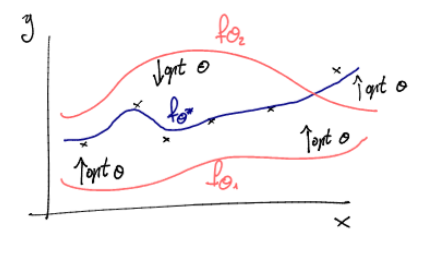
\includegraphics[width = .7\linewidth]{images/optimization}
\caption{Optimization process of a machine learning algorithm. The model is capable of representing many functions (in red), which are optimized to fit the existing training data (in blue). }
\label{fig.optimization}
\end{figure}

There exist a plethora of algorithms to solve optimization problem, and in general no optimization algorithm is capable of solving all of them, even approximately. Among the available options, one can distinguish simplicial algorithms (Nelder-Mead \cite{nelder1965simplex}), evolutionary algorithms (CMA-ES \cite{hansen2006cma}) or gradient-based approach to first or higher orders \cite{kingma2017adam, byrd1995limited, nocedal2006fundamentals}. 

In particular, neural networks admit the use of \textit{backpropagation} as an optimization algorithm. This enables using neural network as a learning method, and lies at the core of machine learning as a product for industrial purposes. Backpropagation will be covered in depth within the scope of this course. 
  
A third relevant ingredient is the generalization. As previously mentioned, the optimization of a machine learning algorithm can only learn the training data. The hope is that this learning is enough to learn also the test or validation data. An interpretation is that the model can actually \textit{learn} the internal properties and structure of the data, instead of just \textit{memorizing} the training data, and not being capable of inferring any information from previously unseen data. The difference between these two quantities is usually called the generalization error, 
\begin{equation}
    \mathcal G(\theta) = \left\vert \mathcal L_{\mathcal D}(\theta) - \mathcal L_{\mathcal T}(\theta) \right\vert,
\end{equation}
usually studied through generalization bounds \cite{wolf2023mathematical}. 

This topic will not be covered in these lectures, hence it is relevant to give some information about it. Generalization bounds capture the complexity of the model, that is, how many choices the training discards. As a consequence, it is possible to know how many training data is needed to narrow the outcomes of the learning algorithm. Intuitively, if the model is too sophisticated, it can learn any kind of data, but also there exist many possible outcomes that correspond to the same data. The training is not capable of knowing which of the outcomes is optimal for unseen data. Hence, the model generalizes poorly. In this case, the model is said to \textit{overfit} the training data.

\section{Types of machine learning}\label{sec.types}

There exist several different types of machine learning algorithm, depending on the input and output of the problem at hand, and the objective of the learning procedure. In this section, we will give a brief description of the most relevant ones, with the goal of providing a comprehensive but not exhaustive overview of the field. 

The different types for machine learning are here organized in an ascending order of lack of knowledge. The less is known about the data, the more unstable and difficult to train the machine learning algorithms become. 

\begin{figure}
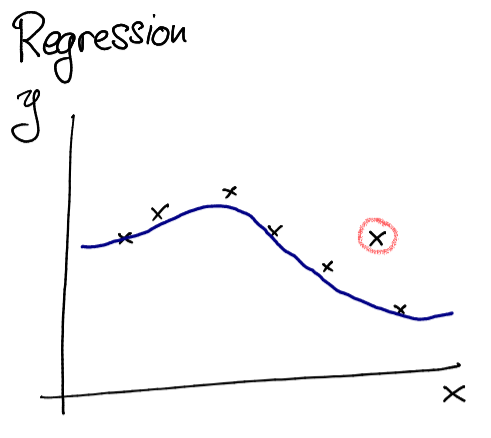
\includegraphics[width = .3\linewidth]{images/regression}
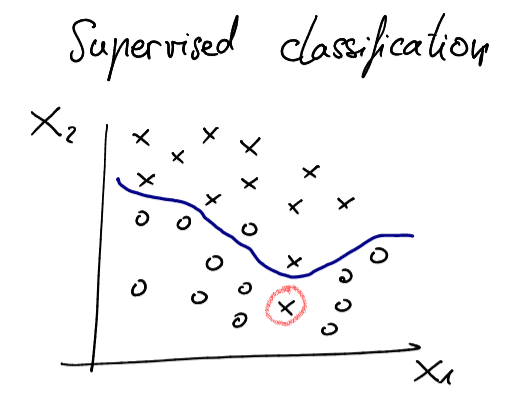
\includegraphics[width = .3\linewidth]{images/supervised classification}
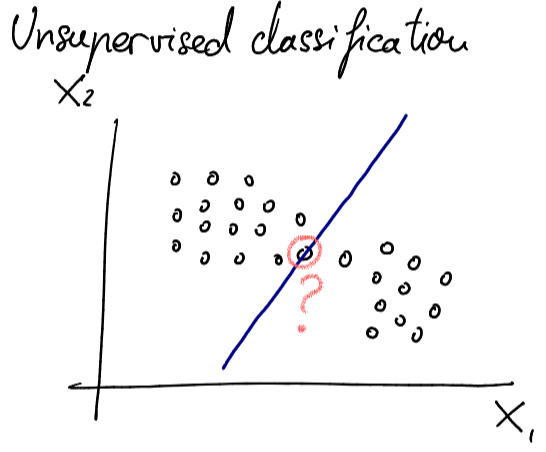
\includegraphics[width = .3\linewidth]{images/unsupervised classification}
\end{figure}

\subsection{Regression}\label{sec.regression}

\begin{figure}



\caption{Different tasks to be addressed with machine learning. In regression, the task is to fit an unknown function known only through data. In supervised classification, the algorithm intends to separate between labeled data, to learn the feature that performs the classification. In unsupervised classification, the goal is to clusterize data, without any prior reference.}
\end{figure}


For solving a regreesion problem in machine learning, consider a function of the form 
\begin{equation}
y: \mathbb{R}^m \rightarrow \mathbb R^n, 
\end{equation}
usually with $m > n$, but not requiredly. The goal is to find a hypothesis function $f_\theta(\cdot)$ such that, for all $x$ in the domain of $f$, 
\begin{equation}
y(x) \approx f_\theta(x).
\end{equation}
The function $f_\theta(x)$ is known as the hypothesis function. A machine learning algorithm is capable of implementing a family of functions 
\begin{equation}
\mathcal H = \{ h_\theta\}_\theta, 
\end{equation}
where each $\theta$ is the label corresponding to each hypothesis function. The functional form of the hypothesis function usually depends explicitly on the parameters. An example of a hypothesis family is
\begin{equation}
\mathcal H_{\rm sin} = \left\{ \sin(x + \theta)\right\}_\theta.
\end{equation}
A machine learning algorithm capable of representing this hypothesis family will be capable of learning sinoidal functions, but will struggle with data that does not correspond to this particular functional form. 
\begin{wrapfigure}{R}{.5\linewidth}
\centering
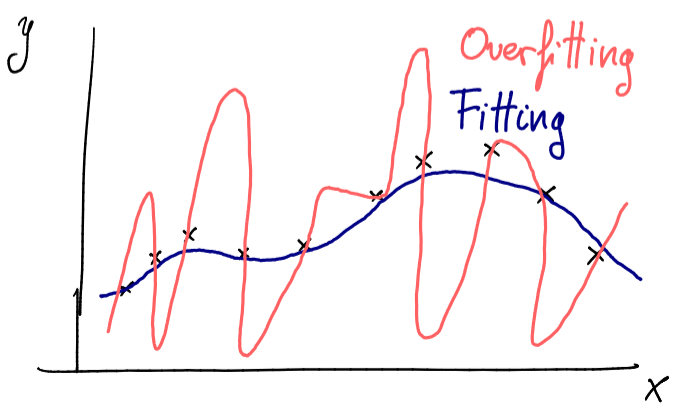
\includegraphics[width = \linewidth]{images/overfitting}
\caption{Overfitting in regression models for machine learning. The overfitted function can reach zero training error on the training data. However, its behavior between these points is unpredictable, yielding to large errors in test data. On the other hand, a fitted function may learn training data only approximately, with the advantage of yielding good approximations for test data. There is no \textit{a priori} manner to know if a model is overfitting, one can only assess that property through testing.}
\end{wrapfigure}

One could agree that machine learning for regression is nothing but statistical regression with a extra steps. Consider for instance the hypothesis family given by
\begin{equation}
\mathcal H_{{\rm poly}, N} = \left\{ \sum_{n = 0}^N a_n x^n \right\}, 
\end{equation}
for $x \in \mathbb R$. For this hypothesis family, it is possible to use $N$ data points to find the optimal configuration of $\{ a_n\}$ to fit the data. Alternatively, one can use $M \gg N$ data points and statistical regression procedures to obtain the configuration minimizing the errors. This model would be capable of representing any polynomial up to degree $d$. Since all analytical functions admit a representation in polynomials by virtue of Taylor's expansion, polynomial regression suffices in principle to approximate any function (within the limits of Taylor's theorem). However, many terms would be needed to approximate functions with slowly vanishing terms. 

While the previous paragraph is always available, it clashes with the spirit of machine learning. Regression techniques as the one explained before requires an \textit{a priori} knowledge of the problem to be solved, sometimes dubbed as an ansatz. Machine learning, and in particular deep learning (to be discussed in \Cref{sec.neural-networks}), generates large hypothesis families with no immediate constructions of their functional forms to automatically look for an optimal solution. 


Regression tasks allow for an immediate interpretation of \textit{overfitting}, a common name for generalization error, see \Cref{ch.introduction}. Machine learning algorithms look for an optimal configuration of its internal degrees of freedom with respect to a training data, and it \textit{hopes} for good performance also in test data. The relevant figure of merit is the accuracy with respect to the unseen data, to ensure \textit{learning} of the internal structure of the data, rather than \textit{memorizing}. Overfitting can be usually prevented by limiting the change rate of the hypothesis functions, usually through regularization cost functions. 


\subsection{Supervised classification}\label{sec.classification}

Supervised classification is a paradigmatic example of machine learning. In many machine learning talks, the subject is introduced as an algorithm capable of telling whether a given picture is a picture of a cat or a dog. In more formal terms, the goal is to receive data that is labelled as belonging to one class out of two (or many). Then, for new data, the algorithm must distinguish the classes among them. 

Supervised classification can be seen as a particular case of regression, restricting the data function to the form
\begin{equation}
y: \mathbb R^n \rightarrow \mathbb Z. 
\end{equation}
One can map the data functions from regression $(y_r)$ to classification $(y_c)$ as follows. Consider the image of $y_r$ being $\mathbb R$. Then, an integer rounding of the output would be enough to perform classification. Alternatively, if the image is $[0, 1]^C \in \mathbb R^C$, the classification can be performed by considering $y_r$ as a step function, doable by rounding functions. 

The paradigmatic example of supervised classification are support vector machines (SVM) (see \Cref{sec.support-vector-machines}). In this method, data points are classified with respect to a hyperplane dividing the data space in two pieces. To this end, the concept of \textit{kernel} arises. A kernel is a function $\phi$ embedding data $x$ into a feature space where the classification is performed. In a nutshell, it is possible to perform classification by just computing inner products between data points (in the feature space), rather than embedding this data into the space. In general, choosing the right kernel $\phi$ is crucial to the performance of the algorith. This acquires special relevance in quantum machine learning, where the first quantum advantages were found for quantum SVMs for well chosen embedding kernels \cite{liu2021rigorous}.

In the references to binary classifications for SVMs, we will only focus on binary classification, as it is usually done in machine learning references. The reason is that it is possible to to combine binary classifiers to create a classifier for larger number of classes $C$. A possible approach is to create a binary classifier for distinguishing $C = 0$ and $C \neq 0$. Then, a second classifier is applied to the data labeled as $C \neq 0$ to classify this data as $C = 1$ or $C \neq 1$. This procedure can be repeated until the end of classes. Another approach is to utilize several classifiers to distinguish $C = i$ or $C \neq i$, for all $i = \{0, 1,\ldots C - 1\}$\footnote{In the notes, I will start the indexing in $0$, to keep consistency with the code in \texttt{Python}.}, and crosscheck the outputs. 

\begin{figure}
\centering
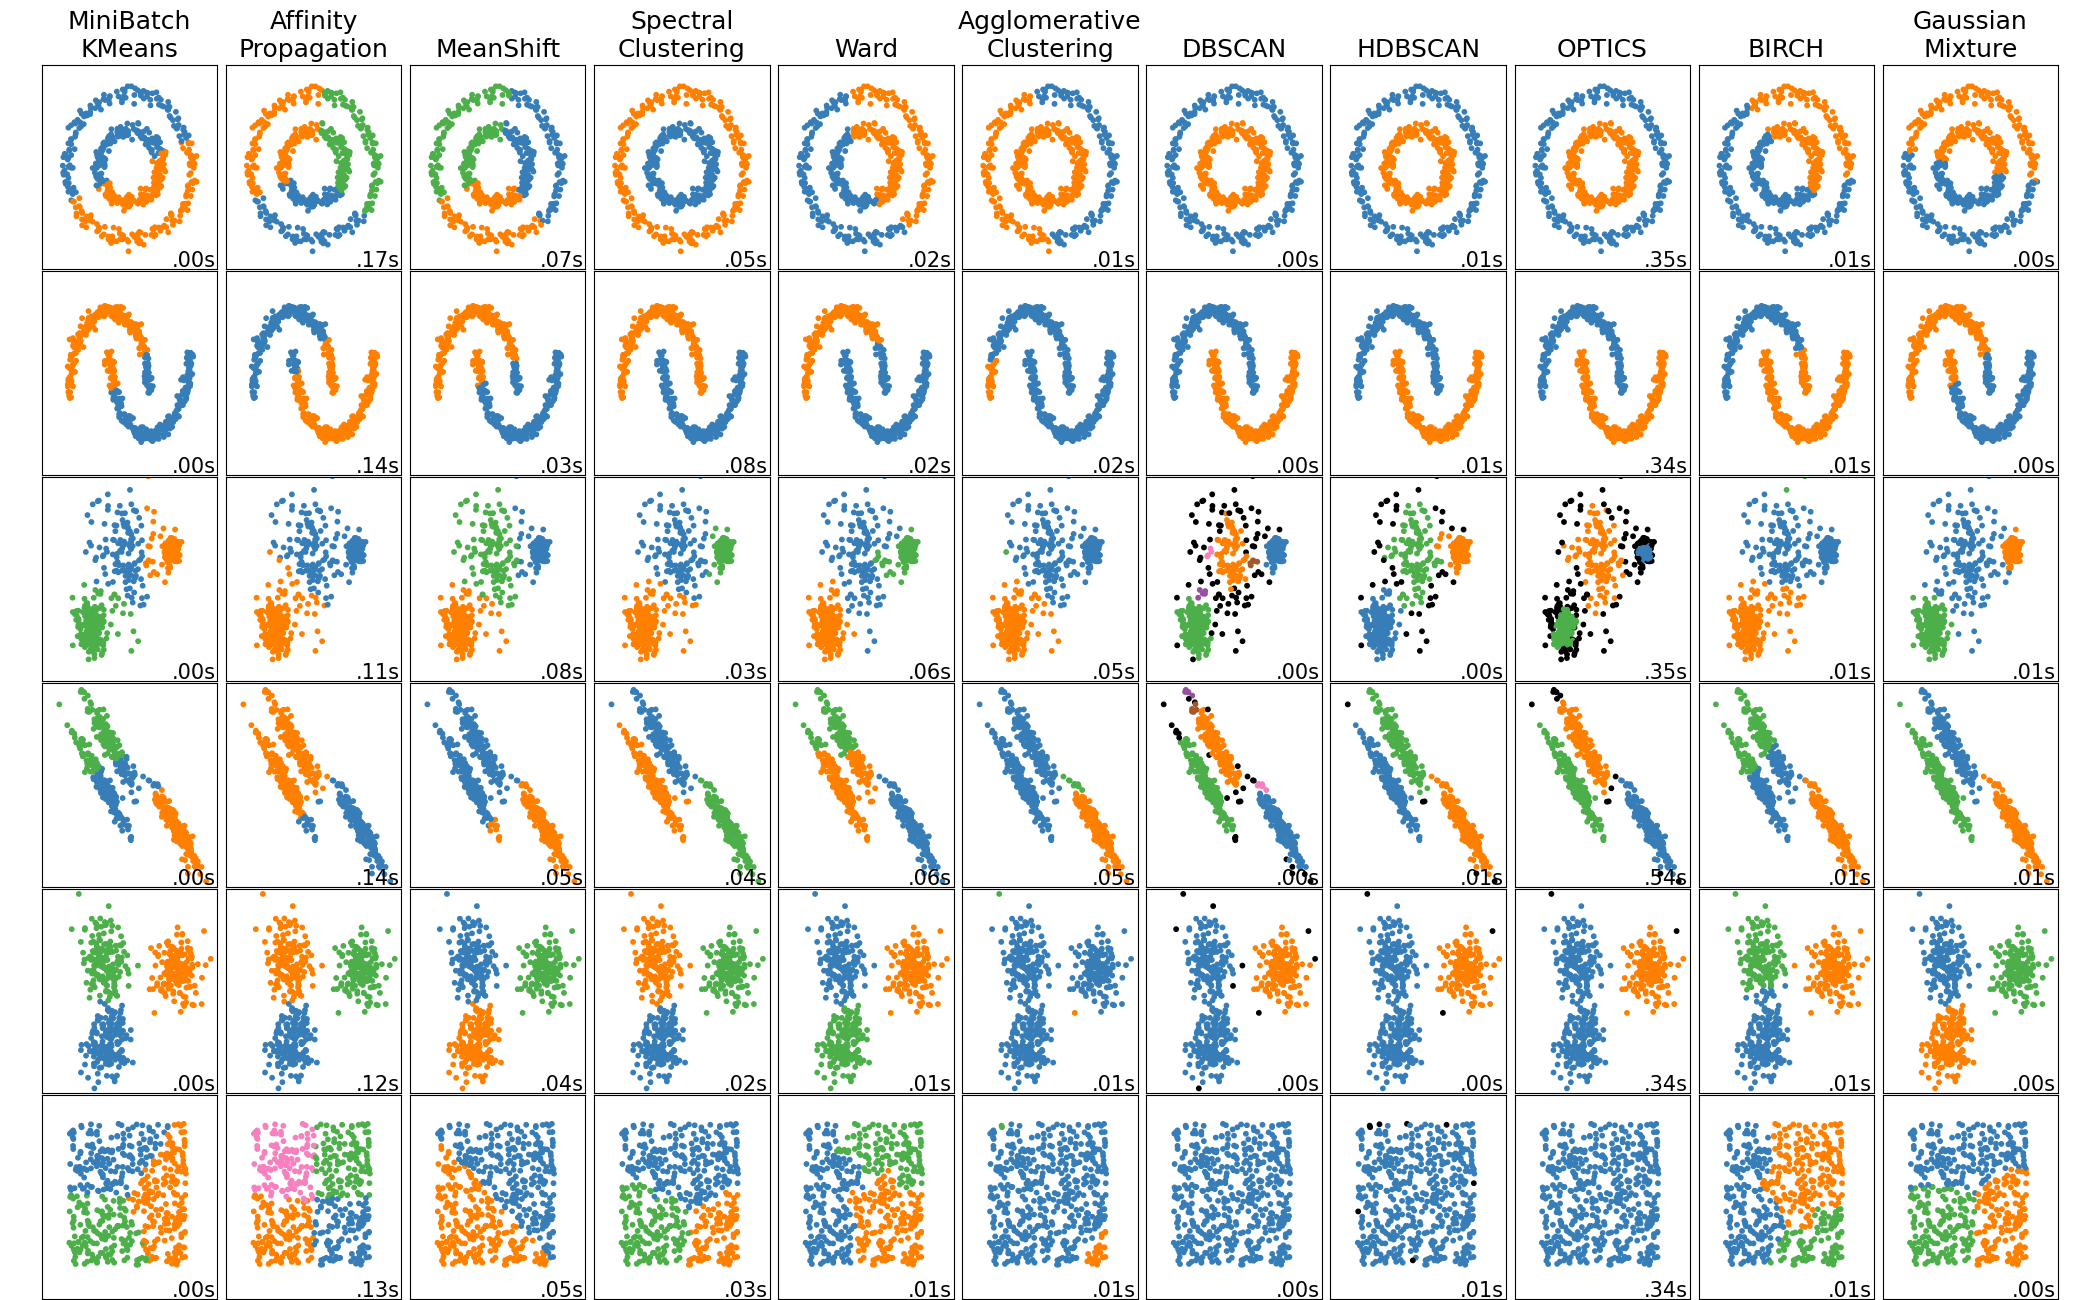
\includegraphics[width = .8\linewidth]{images/cluster_datasets}
\caption{Example of data and proposed solutions by different algorithms for a supervised learning problem \cite{pedregosa2011scikitlearn}. The data does not provide any information on how go distinguish between classes or even how many classes one should consider. Thus, this information has to be input into the algorithm by the user, yielding different results. }
\label{fig.unsupervised-learning}
\end{figure}

\subsection{Unsupervised classification}\label{sec.unsupervised-classification}

Unsupervised classification, also known as clustering, is the learning algorithm of dividing data in several classes, based on the internal structure of the data. In this case, there is no right answer, since the data does not provide a \textit{true labelling}. In unsupervised learning, the performance can only be assessed with respect to the input of data, and not with respect to the output. Hence, unsupervised classification crucially depends on the quality of the data, not only on the capabilities of the learning procedure. 

Consider the example here given in \Cref{fig.unsupervised-learning}. Visually, it is obvious that data can be divided in two classes. If the two \textit{moons} are located one distant away from the other, a SVM together with euclidan distance should suffice to provide an accurate discrimination. In contrast, if the \textit{moons} are located close to each other, it would be necessary to introduce a appropriate data embedding to ensure linear classification. 



Unsupervised learning will not be exhaustively covered in these notes. However, good references can be found in \cite{pedregosa2011scikitlearn}.

\subsection{Generative modelling}

Generative modelling is a subfield of machine learning consisting in obtaining a model from which it is possible to sample data that resembles some other training data. 

Consider a model $\mathcal A$ that is capable of outputting random variables of the form
\begin{equation}
x \sim \mathcal D_{\mathcal A}, 
\end{equation}
where $\mathcal D_{\mathcal A}$ is a probability distribution specified by the machine learning algorithm, either by its architecture or by its parameters. 

The random variable $x$ is intended to be indistinguishable (or at least close enough) to some other training data, that is
\begin{align}
x_t & \sim \mathcal D_T \\
x_t & \sim \mathcal D_{\mathcal A} \\
\mathcal D_T & \approx \mathcal D_{\mathcal A}.
\end{align}
Hence the task is to approximate $\mathcal D_{\mathcal A}$ as much as possible to $\mathcal D_T$. 

There exist several manners to sample random variables from a specified probability distribution. A simple way is to generate a function 
\begin{equation}
f: \mathbb R^m \rightarrow \mathbb R^n, 
\end{equation}
and then apply $f$ to a random variable sampled from a simple probability distribution. For example, consider $z \in \mathcal N(0, 1)$, with $\mathcal N$ being a Gaussian distribution. Then, we define
\begin{equation}
x \equiv f(z) \sim \mathcal D_{\mathcal A}, 
\end{equation}
and the generative modeling problem can be understood as a re-interpretation of a regression problem, with a modified cost function. 

Alternatively, one can define a model that generates samples instead of transforming a random variable. Consider for instance a binary decision tree. Each new branch can take two possibilities, namely 0 or 1, at random. At the end of the tree, the model returns the followed path, which is completely specified by a bitstring of 0's and 1's. Each bitstring will be sampled with different probability, depending on the model itself. In a side note, these decision-based algorithms can only return integer numbers, which can approximate real numbers to arbitrary accuracy. 
\begin{wrapfigure}{R}{.5\linewidth}
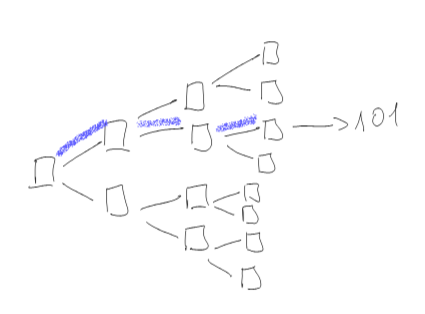
\includegraphics[width = \linewidth]{images/decision-tree}
\caption{Example of a sampling model based on decision diagrams. }
\label{fig.decision}
\end{wrapfigure}


A strong difficulty of generative modelling is that it is not possible to have access to the probability distributions from which data is sampled, either for training (as discussed before) or for generated data (since the possibilities are usually very large). Hence, one cannot rely on exhaustive descriptions of the data, but only on approximate descriptions that \textit{hopefully} will suffice to solve the problem at hand. The same argument holds to compare target and obtained probability distributions. Measuring the distance between these distributions is in general difficult, hence imaginative methods have been developed, such as adversarial training or approximated distances, to be discussed in \Cref{sec.generative-tensorflow}. 

In spite of all the formal and theoretical problems that arise in generative models, this branch of machine learning / artificial intelligence has exhibited a strong development in recent years, being ChatGPT or Dall-E the most celebrated examples. Since these algorithms are capable of \textit{mimicking} existing probability distributions, they excel at outputting samples of material that is well-known, for example tax forms, cover letters, or human faces. However, these models struggle when generating data which is significantly different from established sources. This is a consequence of data being impossible to sample exhaustively. 

\subsection{Reinforcement learning}

In reinforcement learning, a machine learning algorithm is trained to interact with some environment and obtain some reward from it. At each step, the machine or \textit{agent} can perform one \textit{action} on the environment. The internal states of the agent and the environment may change. The action will return some \textit{reward} on the agent, awarded by the \textit{interpreter}, which can be constructed from data. The goal of the agent is to perform the sequence of actions that maximizes the obtained reward from an environment. 
\begin{wrapfigure}{R}{\linewidth}
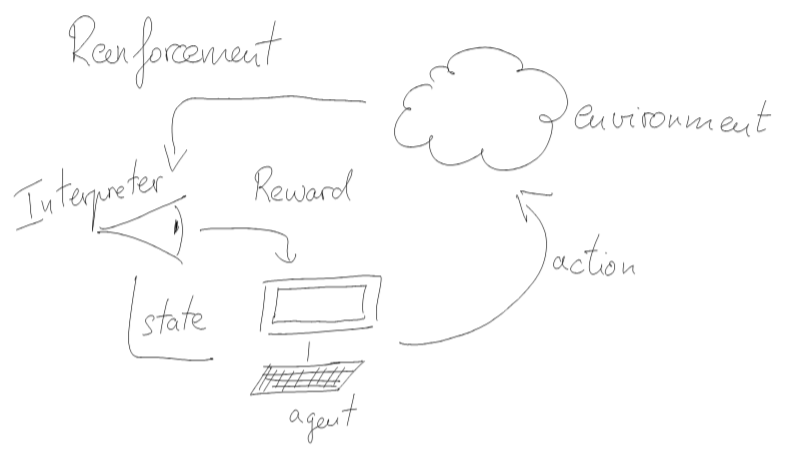
\includegraphics[width = \linewidth]{images/reinforcement-learning}
\caption{Scheme for reinforcement learning}
\label{fig.reinforcement-learning}
\end{wrapfigure}

As an example, consider playing chess. The machine is initially equipped with the basic moves of the pieces. The agent is one player, and the environment is the opponent. The interpreter is composed by large data samples on previous matches played by humans. The machine moves one piece (takes one action) and the environment responds with another move. The position of the board can be compared to a stored database to estimate the probability of each player to win. Over time, the machine learns to play chess intelligently, by just imitating those moves that maximize the winning probability. 


\chapter{Regression and supervised classification}

In this chapter we will cover the basic of regression and supervised classification, both theoretical notions (not so much) and numerical examples. We will create the models from scratch, to give ideas of what we are doing and why. We will cover neural networks (NN) and also support vector machines (SVM). These models are at the very core of machine learning. 

\section{Neural networks}\label{sec.neural-networks}

Neural Networks (NN) are arguably the most relevant models in machine learning, and have been widely implemented to solve large varieties of problems. NNs are mathematical constructions with three main properties, which make them ideal to address machine learning tasks.

\begin{itemize}
\item \textit{Expressivity:} NNs are models with large representation capabilities, that is, they can represent many different functions to accommodate arbitrary data. This implies that the models of the same form, possibly with different sizes, can be used to solve many different and complicated problems. 
\item \textit{Trainability:} Apart form the expressive capabilities of NNs, its inner structure allows for an efficient training algorithm based on gradient optimization. Computing the gradients of the output functions of the NN with respect to their internal degrees of freedom is \textit{efficient}, that is, it does not require any overhead with respect to computing the function itself. Hence, it is possible to find the optimal configuration of the NN with relatively small effort. 
\item \textit{Linear algebra:} NN are based on matrix multiplication and application of easy functions repeatedly. This property allowed for the development of specific hardware, in particular GPUs, that are specifically suited to evaluate NNs, by accelerating matrix multiplication. The specific hardware, together with dedicated software and computational methods allowed for large-scale implementations of NN that have already revolutionized information processing. 
\end{itemize}

\subsection{What are neural networks}\label{sec.what-neural-networks}
The mathematical structure of NNs is very simple. It is based on a feedforward mechanism that transports data from an input layer to an output data. 

Let us consider first the single-layer neural network. The input data $x \in \mathbb R^m$ is input to the model through an input layer of $m$ neurons. Then, this data is transferred to a middle (hidden) layer composed by $h$ neurons. The input to any of these neurons is given by a linear combination of the input data as $w \cdot x + x_0$. This neuron then applies an \textit{activation function}, $\sigma(\cdot): \mathbb R \rightarrow \mathbb R$. Hence, the output of the hidden layer is given by
\begin{equation}
f_h(x) = \sigma_h(W_h x + b), 
\end{equation} 
with $W_h \in \mathbb R^{h \times m}, b \in \mathbb R^h$. The matrix of \textit{weights} $W_h$ and the \textit{biases} $b$, together with the activation function, define the hidden layer. In a neural network with several layer, each weights matrix and bias, and each activation function are independently chosen. 

For the output functions, the procedure is repeated, yielding
\begin{equation}
f(x) = \sigma_o(W_o \sigma(W_h x + b_h) + b_o).
\end{equation}
This single-layer neural network suffices to provide an extremely rich hypothesis family, in fact \textit{universal}, that is capable of representing any function. This is supported by the universal approximation theorem, see \Cref{sec.universality-nn}. 

\begin{figure}
\centering
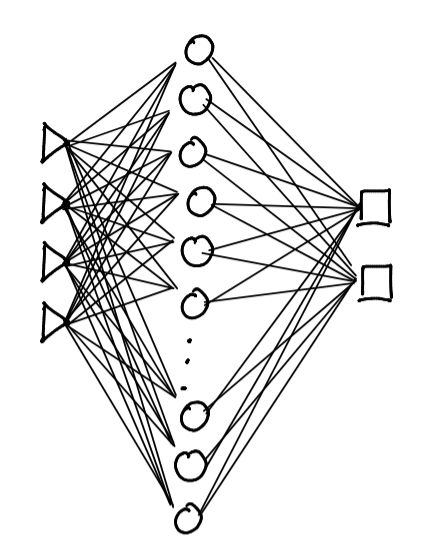
\includegraphics[height = .475\linewidth]{images/single layer nn}
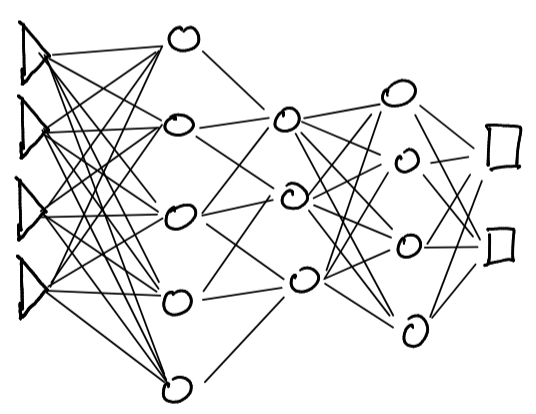
\includegraphics[height = .475\linewidth]{images/multilayer nn}
\caption{Single-layer and multilayer neural networks. Both models are universal, i. e., the output function (square) can be any function of the input (triangles). However, in practice, deep neural networks provide better processing layers than single layer. }
\label{fig.neural-network}
\end{figure}

From the single-layer NN, it is immediate to construct a more sophisticated model known as deep neural network. Consider the same structure as explained in the single-layer neural network. The deep neural network is simply given by
\begin{equation}
f(x) = \sigma_L(b_L + W_L \sigma(b_{L-1} + W_{L - 1} \sigma(b_{L-2} + W_{L - 2} \sigma_{L - 2}(\cdots\sigma(b_1 + W_1 \sigma(b_0 + W_0 x)) \cdots)))).
\end{equation}
The definition of the NN creates an easy to evaluate and represent function with properties that are hard to characterize from an analytical point of view. Hence, the use of computational tools is a crucial element to study neural networks. 

\subsection{Universality of neural networks}\label{sec.universality-nn}

\paragraph{Universal approximation theorem (UAT) \cite{cybenko1989approximation} --}Consider a NN where $\sigma_o(\cdot)$ is the identity function, and $n = 1$. Consider the activation function $\sigma_h(\cdot)$ to be any continuous sigmoidal function, that is 
\begin{align}
\lim_{x \rightarrow -\infty} \sigma(x) = 0 \\
\lim_{x \rightarrow \infty} \sigma(x) = 1.
\end{align}
Then, for every continuous function $
y:[0, 1]^m \rightarrow \mathbb R$, there exists a value of $h$ such that, for every $\epsilon > 0$, 
\begin{equation}
\max_{x \in [0, 1]^m} \left\vert y(x) - f(x)\right\vert \leq \epsilon.
\end{equation}
This is known as \textit{uniform approximation}, implying that for any point $x$ the approximation can be made arbitrarily small. 

It is important to mention that this version of the theorem applies with some restrictions, specially in the choice of activation functions. However, it is possible to extend this result to more general situations, for example by using bounded, non-constant and continuous functions. In particular, we choose $\sigma(\cdot) = \cos(\cdot)$ to discuss the differences between NN and other representation theorems. 

Consider the Fourier theorem, stating that any periodic square-integrable continuous function $y$, that is satisfying
\begin{equation}
\Vert y(x) \Vert_2 \equiv \int_{x \in [0, 1]^m} \vert y(x) \vert^2 dx < \infty,
\end{equation}
can be approximated by a function of the form\footnote{Note that here $n \in \mathbb Z^m$, although the vectorial nature is not specifically mentioned. }
\begin{equation}
f_N(x) = \sum_{\Vert n \Vert_1 \leq N} c_{n} \cos(n \cdot x) + s_{n} \sin(n \cdot x), 
\end{equation}
with 
\begin{align}
c_n = \frac{1}{(2\pi)^m} \int_{[0, 1]^m} \cos(n \cdot x) y(x) \\
s_n = \frac{1}{(2\pi)^m} \int_{[0, 1]^m} \sin(n \cdot x) y(x)
\end{align}
to an error 
\begin{equation}
\Vert f_N(x) - y(x) \Vert_2 = \left \vert \Vert y(x) \Vert_2 - \sum_{\Vert n \Vert_1 \leq N} \vert c_n\vert^2 + \vert s_n\vert^2\right\vert.
\end{equation}
The intuition behind Fourier's theorem is as follows. The functions $\sin$ and $\cos$ constitute a basis in the space of square-integrable functions, including but not limited to continuous functions.  This space is infinite-dimensional and equipped with the inner product
\begin{equation}
\langle f, g \rangle = \frac{1}{(2\pi)^m} \int_{x \in [0,1]^m} f(x) g^*(x) dx .
\end{equation}
In the language of linear spaces, Fourier's theorem simply decomposes the function of interest in a basis of the space of functions, and creates a finite-dimensional representation of $y$. Since this function is square-integrable, the approximation obtains better accuracies as $N$ increases. 

The UAT, in its $\sin / \cos$ form, can be rewritten as 
\begin{equation}
f_h(x) = \sum_{i = 1}^h c_{i} \cos(w_i \cdot x) + s_{i} \sin(w_i \cdot x). 
\end{equation}
The elements that construct this approximation have tunable weights. Each of these elements, for $w_i \in \mathbb R^m$ has a non-zero overlap with the basis elements $\sin(n \cdot x), \cos(n \cdot x)$. The immediate consequences, proven by UAT, is that NNs densely cover the space of continuous functions, in the supremum norm, due to the freedom in the weights. Additionally, note that the number of degrees of freedom scales as $h \times m$, while in the Fourier theorem, this number scales as $N^m$.

Extensions to UAT were proven for more general versions of single-layer NNs and also for deep NNs \cite{hornik1991approximation}. This collection of results theoretically supports the use of NNs for machine learning, but they do not justify \textit{in practice} their widespread implementation for solving many different kind of problems. The usage is usually motivated by continuous good performance on the considered models on almost any task. 

\subsection{Training of neural networks: backpropagation}

We address now backpropagation, the most celebrated method to train NNs. The optimization process usually relies on gradient-based methods. For those methods to be used, it is required to estimate or compute the gradients of the neural networks, with respect to the internal degrees of freedom, namely weights and biases. 

The framework of interest is as follows. Consider a loss function
\begin{equation}
\mathcal L_{\mathcal T}(W, b)= \frac{1}{\vert \mathcal T \vert} \sum_{x \in \mathcal T} D(y(x) - f_{\rm NN}(x)), 
\end{equation}
for $D(\cdot, \cdot)$ being a distance, for example the mean squared error. We are interested in computing
\begin{align}
\frac{\partial \mathcal L_x}{\partial W_l} = \frac{\partial D(y(x), f_{\rm NN}(x))}{\partial f_{\rm NN}(x)} \ \frac{\partial f_{\rm NN}(x)}{\partial W_l}\\
\frac{\partial \mathcal L_x}{\partial b_l} = \frac{\partial D(y(x), f_{\rm NN}(x))}{\partial f_{\rm NN}(x)} \ \frac{\partial f_{\rm NN}(x)}{\partial b_l}\\
\end{align}
where the subindex $x$ states the loss function evaluated in one data point. Aside from a small weight given by the distance function, the most relevant part is given by the derivatives of the NN with respect to the internal parameters. For the last layer, we can immediately compute the derivatives as $\delta_L$. This quantity can be used to \textit{backpropagate} the effect of training data on the derivatives with respect to the biases as
\begin{align}
\frac{\partial f_{\rm NN}(x)}{\partial b_L} = \sigma^\prime \odot \frac{\partial f_{\rm NN}(x)}{\partial \sigma_L} \frac{\partial D(y(x), f_{\rm NN}(x)}{\partial y(x)} \\
\frac{\partial f_{\rm NN}(x)}{\partial b_{l - 1}} = \sigma_{l - 1}^\prime \odot (W_l)^T \frac{\partial f_{\rm NN}(x)}{\partial b_l}, 
\end{align}
with $\odot$ being a elementwise multiplication.
The corresponding derivatives with respect to weights is just given by
\begin{equation}
\frac{\partial f_{\rm NN}(x)}{\partial W_l} = \frac{\partial f_{\rm NN}(x)}{\partial b_l} \left(\sigma_{l - 1}\right)^T,
\end{equation}
with $\sigma_l(x)$ being the output of the $l$-th layer of the NN. 

The most important implication of backpropagation is that it is possible to compute the gradients with no extra cost as compared to evaluating the NN itself, up to matrix multiplication. 

\subsubsection{Stochastic Gradient Descent}

Backpropagation is usually combined with stochastic gradient descent (SGD). This is nothing but computing average gradients over data, when the data is splitted in \textit{batches}, and these batches are chosen at random. SGD favors training due to statistical fluctuations of the data, preventing the algorithm from being trapped in local minima of the optimization landscape. 

\subsection{Types of neural networks}

There exist many different models on neural networks in the literature, that have been proposed and developed with the goal of efficiently addressing some particular problems. In this chapter we give an overview of them, with no aim to be exhaustive. 

\subsubsection{Activation functions}

In practice, NNs can work with almost any kind of activation function that one can imagine. However, some examples have been more extensively used than other. 

\paragraph{Sigmoid --} The sigmoid function is one of the most used activation functions in NNs. It is defined as
\begin{equation}
\sigma(x) = (1 + e^{-x})^{-1}.
\end{equation}
The name \textit{sigmoid} can provoke confusions with the notion of sigmoidal functions mentioned in~\Cref{sec.universality-neural-networks}. In the theorem, a sigmoid function is just a function satisfying the conditions there specified. The choice here given fulfills those requirements, but it is a specific example. 

This function has the property that
\begin{equation}
\frac{\partial \sigma(x)}{\partial x} = \sigma(x)(1 - \sigma(x)), 
\end{equation}
hence the back propagation algorithm can benefit from this choice to further reduce the computational cost of computing the derivatives. 

\paragraph{ReLU --}
The ReLU function is defined as
\begin{equation}
\operatorname{ReLU}(x) = \max(0, x).
\end{equation}
Interestingly, this function does not fulfill the requirements of sigmoidal functions specified in \Cref{sec.universality-neural-networks}. However, this can be solved by creating the function
\begin{equation}
g(x) = \frac{1}{\vert b - a\vert } \left(\operatorname{ReLU}(x - a) - \operatorname{ReLU}(x - b)\right), 
\end{equation}
with does fulfill the sigmoid conditions. 

\begin{figure}
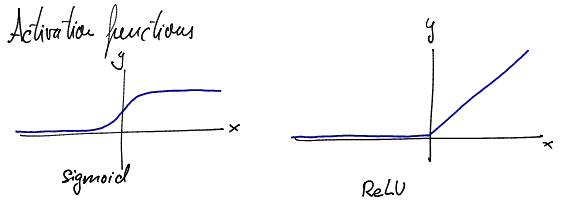
\includegraphics[width = .7\linewidth]{images/activation functions}
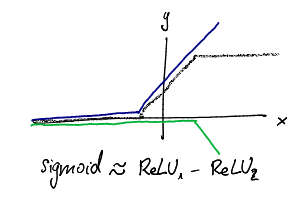
\includegraphics[width = .35\linewidth]{images/sigmoid relu}
\end{figure}

There is a more relevant reason to use ReLU functions, derived from the vanishing gradients problems. Recalling back propagation, it is noticeable that the size of the derivatives scales as $(\sigma^\prime)^L$, for fixed values of the weights. Hence, if $\sigma^\prime \vert \leq 1$, the derivatives on the first layers are suppressed as compared to the last layers. In particular, the sigmoid function previously defined has derivatives close to zero in most of its domain, with the exception of the region around $x = 0$. By applying the ReLU function, these derivatives are constanly 1, avoiding the vanishing gradients problems. 


\subsubsection{Exotic neural networks}

The NN previously explained is known as feedforward fully connected NN, and has all the relevant properties that make NNs unique. However, there exist many more examples of NNs. 

\paragraph{Recurrent NNs --} These networks propagate data not only forward, but also within the same layer, see \Cref{fig.recurrent-network}. Recurrent NNs are particularly useful for sequential data processing, in which the data of time step $t$ depends on the output of step $t - 1$. 

\begin{figure}
\caption{Recurrent neural network}
\label{fig.recurrent-network}
\end{figure}

In the recurrent NN, the neurons have some internal memory, equivalent to the weights and biases in the feedforward NN, that is updated at every time step based on the input and its previous state. The memory keeps information from previous state and incorporate knowledge. There exists a variant of recurrent NNs named long-short term memory (LSTM) that solves the problem of vanishing gradients in recurrent NNs. 


\paragraph{Convolutional NNs --} Convolutional layers apply geometrical kernels, that is, a given fraction of the input is convolved with a given kernel, and the output is stored in the next layer, as
\begin{equation}
\operatorname{ConvNN_w(x)}_i = \sum_{j} w_j x_{i + j}.
\end{equation}
These NNs are particularly useful to process data in the form of images, since they are capable of extracting geometrical features of the input data. One can freely choose how the convolution is applied to optimize the performance of the model for the problem of interest. 

\paragraph{Autoencoder --}An autoencoder is a network that effectively reduces the dimensionality and complexity of the input data. Any kind of netowrk or layer here explained can be used to this purpose. The autoencoder is composed of two elements, namely the encoder and the decoder. The encoder received input $x$ and outputs a succinct description of it. The decoder receives the succinct description and reverts the compression to obtain and output $x^\prime$. If $x \approx x^\prime$, then the decoder efficiently learns a dimensionality reduction of the input $x$. 

Autoencoders can be used mainly in two tasks. First, one can consider large data to be compressed into a more simple representation. Since the simple representation is assumed to have the same information as raw data, it can be used as an input to another network to solve a learning problem. The cost of the network is reduced in this way. Second, one can generate data by inputing data in the compressed format to the decoder, creating a generative model. 

\paragraph{Hopfield network --} This network is a form of recurrent NN inspired by physics, in particular by spin glass systems. The Hopfield NN can be interpreted as a network in which neurons interact with each other, rather than acting on the input and feedforward it to the next layer. The Hopfield network provides memory, that is, its internal configuration evolves towards a ground state energy that stores patterns on training. 

The Hopfield network is designed by
\begin{equation}
y_i = \operatorname{sign}\left(\sum_j w_{ij} x_j - b_i\right), 
\end{equation}
and they are designed to store information. If $x$ is a corrupted state or a partial description of it, the Hopfield network will recover the memorized state. Convergence is not guaranteed. 

Hopfield won the Nobel prize in Physics in 2024.

\paragraph{Boltzmann machine --} The Boltzmann machine is inspired by Physics. Consider an Ising model as
\begin{equation}
H_{w, b}(x) = - \sum_i b_i x_i - \sum_{i, j} w_{i, j} x_i x_j, 
\end{equation}
with $x$ being a boolean function. The weights and biases allows us to encode a probability distribution over the boolean functions given by 
\begin{equation}
P(x) \propto \exp(- H_{w, b}(x)). 
\end{equation}

Boltzmann machines distinguish between visible and hidden units. This implies that one can use more than only weights and biases to model the output of the model. Additionally, these hidden units can be used as seed for randomness in generative models. 

An interesting subclass of Boltzmann machines are restricted Boltzmann machines, which only allow for interactions between hidden and visible units, not inside the two components. These models have more efficient training algorithms. 

\begin{figure}
\centering
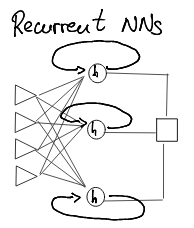
\includegraphics[width = .30\linewidth]{images/recurrent nn} \hskip2cm
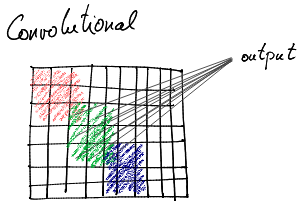
\includegraphics[width = .45\linewidth]{images/convolutional nn}
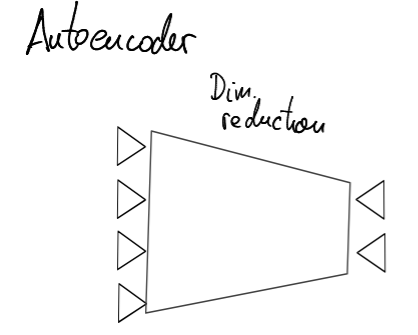
\includegraphics[width = .45\linewidth]{images/autoencoder}
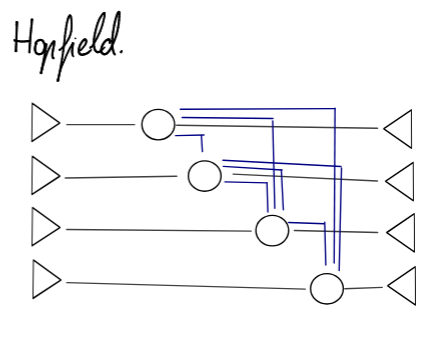
\includegraphics[width = .45\linewidth]{images/hopfield nn}
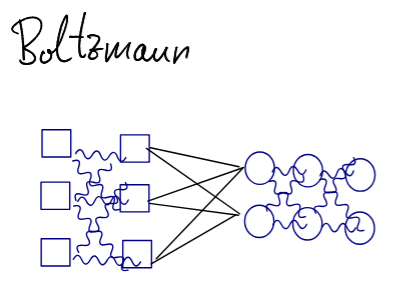
\includegraphics[width = .45\linewidth]{images/boltzmann}
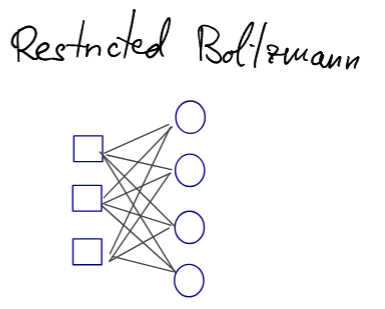
\includegraphics[width = .45\linewidth]{images/restricted boltzmann}
\end{figure}

\subsubsection{Layers}

The previously mentioned networks and activation functions can, in principle, be combined at will to generate customizable neural networks tailored made for specific purposes. Those can also be combined with generic layers with particular effects. 

The rational behind these layers is to remove sophistication of data that contributes redundantly to the learning process. This way, overfitting is prevented, and the training process  is made less costly and easier to converge. Some examples are as follows. 

\paragraph{DropOut --}
The DropOut layer randomly transforms features of the input to zero, or some other fixed or random value. The DropOut layers usually permit any kind of configuration. 


\paragraph{Average --} As denoted by the name, an average layer simply averages over partial descriptions of the inputs. 

\paragraph{Pool -- }A pooling layer samples from the input, for instance by randomly selecting features or retrieving the maximal value. 


\subsection{Creating our own neural network}

For this section, I refer the reader to the Jupyter Notebook available \href{}{here}.

\subsection{Final remarks}

In this section we have reviewed the basic of NNs, as well as some practical considerations for using them as machine learning algorithms. 

The functioning principles of NNs can be understood from analytical considerations, such as the universality theorems and the backpropagation algorithm. Componentwise, it is also possible to acquire certain intuition on how each of them works. However, when all the elements are merged together (see \Cref{sec.tensorflow}), all intuition is lost, and it is really difficult to keep track of the internal processes of data within the network. This question gave rise to the problem of interpretability of machine learning, meaning \textit{what are the processes that a NN carries out to extract knowledge from data}. 
Hence, numerical investigation has been a relevant tool to benchmark the performance of NNs in practice. 

\section{Support vector machines}\label{sec.support-vector-machines}

Support Vector Machines (SVM) are a widely spread machine learning model with applications mainly on binary classification tasks. SVM are, in a nutshell, the process of finding the optimal frontier that linearly separates some data in two classes. The performance of any SVM depends on the properties of the data, or in available transformations that performs non-linear maps on the existing data. 

There is a strong approach difference between SVMs and NNs. The functioning principle of NNs is to build a large pool of models that are efficient to optimize through gradient descent methods. This set of model is such that many possible solutions are available, and the difficulty is to find which one, among all possibilities, is optimal or close to optimal with respect to the training dataset. That is, NNs are models that do not require any a priori knowledge of the task to be solved, and the learning is conducted in an automatic fashion. 

In contrast, SVMs do not properly \textit{learn} the data, but rather they find the optimal separation by finding the solution to a quadratic optimization problem. Hence, it is required that information from the dataset is available, to construct a SVM with the possibilities to perform the required classification. 

\subsection{Binary classification of data}

We address now the problem of using a SVM to binary classify data. Consider data in the form $\mathcal D = \{(x_i, y_i)\}_i$, with $x \in´ \mathbb R^m$, and $y \in \{-1,1\}$. The goal of the SVM is to find a hyperplane that finds the optimal separation of data among classes. Such hyperplane is defined by a weights vector $w \in \mathbb R^m$, and bias $\mathbb b$. The classification is then given depending on whether the data point $x$ is located at one side or the other with respect to the hyperplane, that is
\begin{equation}
y(x) = \sign\left( w \cdot x - b \right).
\end{equation}
Among the SVMs, we can distinguish two different cases, mainly hard- and soft-margin classifiers. 

\begin{figure}
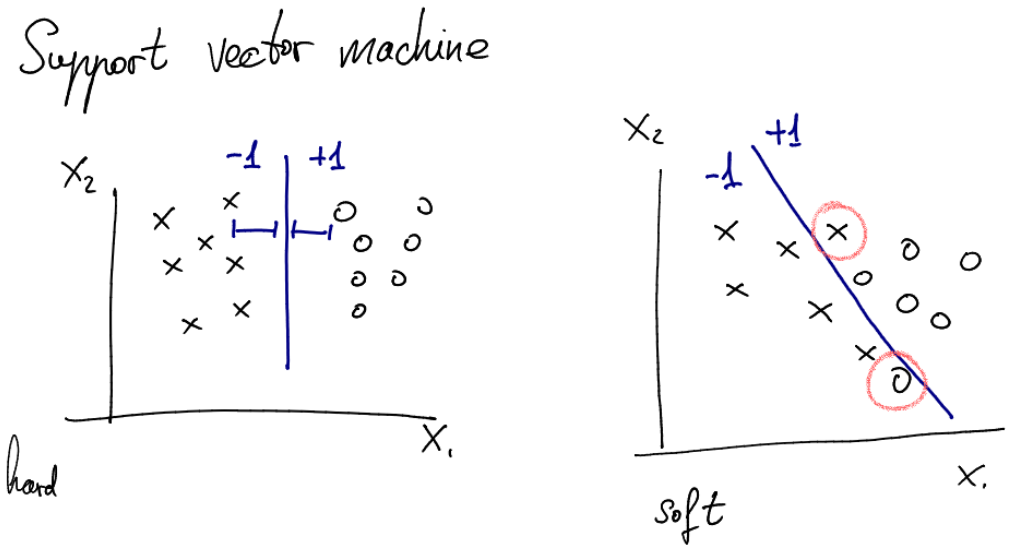
\includegraphics[width = .9\linewidth]{images/SVM}
\caption{Support Vector Machines. The algorithm is capable of finding the optimal linear separation between labelled classes within the training dataset. }
\label{fig.svm}
\end{figure}

For hard-margin classifiers, the data must be linearly separable, and by assumption there exists a hyperplane that correctly classifies all data. This implies that there exist values for $w, b$ such that
\begin{equation}
\forall x: \; y(x) (w \cdot x - b) \geq 1.
\end{equation}
In the case of soft-margin classifiers, the goal is to minimize the loss function
\begin{equation}
C_{\mathcal T}(w, b) = - \frac{1}{\mathcal T}\sum_{x \in \mathcal T} \max\left(0, y(x) \left(w \cdot x - b \right)\right).
\end{equation}
It is common practice to add a regularization term on $\Vert w \Vert$, yielding
\begin{equation}
w, b = \operatorname{argmin}_{w, b} \lambda \Vert w \Vert^2_2 + C_{\mathcal T}(w, b).
\end{equation}
The regularization term is added to the optimization to enhance the generalization capabilities of the model. By limiting the sizes of $w$, it is only possible to find compromises between all data points to find the optimal classification. This optimization is referred to as the \textit{primal} optimization of SVM. 

It is interesting to find the solution of the optimization problem finding the \textit{dual} optimization of the same problem. This duality is a consequence of Lagrangian optimization. Solving problems of the form
\begin{align}
{\rm minimize} & \quad f(w) \\
{\rm subject\, to} & \quad g_i(w) \leq 0 
\end{align}
is equivalent, via Lagrangian multipliers, to solving the problem
\begin{align}
{\rm maximize} & \quad f(w) + \sum_i c_i g_i(w) \\
{\rm subject\, to} & \quad \nabla f(w) + \sum_i c_i \nabla g_i(w) = 0.
\end{align}
In our case, we can identify
\begin{align}
f(w) & = \Vert w \Vert^2 \\ 
g_i(w) & = y_i(w \cdot x_i - b) - 1.
\end{align}
The dual optimization is then 
\begin{equation}
\min_{w, b} \max_{c \geq 0} L(w, b; c) \equiv \min_{w, b} \max_{c \geq 0} \lambda \Vert w \Vert^2 - \sum_i c_i y_i (w \cdot x_i + b) - 1.
\end{equation}
Taking derivatives with respect to the internal degrees of freedom, we can obtain the constraints
\begin{align}
\partial_w L(w, b; c) = 0 & \rightarrow w = \frac{1}{2\lambda} \sum_i c_i y_i x_i \\
\partial_b L(w, b; c) = 0 & \rightarrow \sum_i c_i y_i = 0, 
\end{align}
which can be introduced into the original problem to find
\begin{equation}
c = \operatorname{argmax}_c\max_{\sum_i c_i y_i = 0, c_i \geq 0} \sum_{i} c_i - \frac{1}{\lambda} \sum_{i, j} c_i c_j y_i y_j x_i \cdot x_j.
\end{equation}
Notice that this new formulation allows to rewrite the optimization problem in terms of the internal products between data points, that is $x_i \cdot x_j$. The hyperplane parameters $w, b$ can be recovered from $c$, if needed. However, the representer theorem allows to predict the class for each new point as
\begin{equation}
y(x_{\rm test}) = \sum_{x_i \in \mathcal T} y_i y_{\rm test} x_i \cdot x_{\rm test} c_i, 
\end{equation}
recovering the weights-bias formulation.

Optimally, the soft-margin SVM will behave as a hard-margin classifier, provided the quality of the data. Would that not be possible, then the SVM finds the hyperplane that maximally separates the data. 
\subsection{Kernel trick}
SVMs are optimal classifiers to find linear separations between classes. However, these methods are not capable of performing any non-linear separations. The kernel trick suffices to incorporate this capability into the SVM framework.


Consider the following classification problem. For $x \in \mathbb R^m$, the class is defined as
\begin{equation}
y(x) = \sign(\Vert x \Vert_2 - R) = \sign\left( \sum_{i} x_i^2 - R\right). 
\end{equation}
There is no value of $(w, b)$ that can perform the correct classification in a SVM framework. However, by changing the relevant space $x \mapsto x^2$, the classification becomes trivial, by finding $w = (1, 1, \ldots, 1), b = R$. 

This transformation is known as the Kernel trick, in which non-linear transformations are applied to the raw data to enhance classification. The map $\varphi(x)$ induces a transformation from the data space to a different feature space. The kernel is defined as
\begin{equation}
k(x_i, x_j) = \varphi(x_i) \cdot \varphi(x_j).
\end{equation}

If this kernel is input to the dual optimization problem, it is immediate to observe that the kernel trick allows to perform linear classification in the space induced by the kernel, which does not need to be linear. 

\begin{figure}
\centering
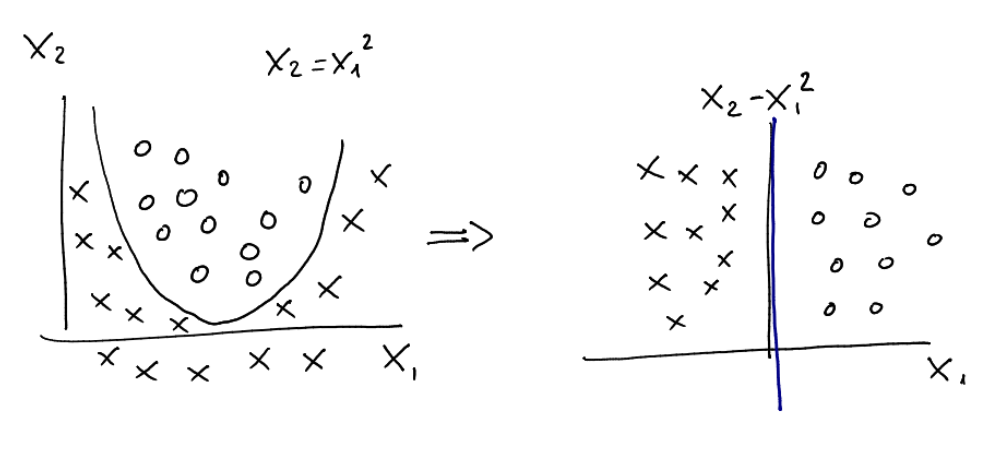
\includegraphics[width = .8\linewidth]{images/kernel trick}
\caption{Description of the kernel trick for the classification of a non-linearly-separable dataset. }
\label{fig.kernel_trick}
\end{figure}


There exist several kernels that are commonly used to perform classification tasks, such as

\paragraph{Gaussian kernel --} This kernel is defined as
\begin{equation}
k(x_i, x_j) = \exp( - \gamma \Vert x_i - x_j\Vert^2), 
\end{equation}
with $\gamma$ being a tunable hyperparameters. This kernel performs well in classification tasks where data corresponding to the same classes concentrate in a relatively small region. The kernel rapidly decays for distances above $\gamma^{-1}$. 

\paragraph{Polynomial kernel --} The kernel is 
\begin{equation}
k(x_i, x_j) = (x_i \cdot x_j)^d, 
\end{equation}
for a given (possibly tunable) given $d$. This kernel suffices to create boundaries that are sensitive to high-order polynomial. 

\paragraph{Sigmoidal kernel --} The this kernel is defined as
\begin{equation}
k(x_i, x_j) = \sigma(a x_i \cdot x_j + b), 
\end{equation}
and also rapidly decays at distances $a^{-1}$ from the bias $b$. 

\paragraph{DLP kernel --} This kernel is useful in quantum machine learning, to demonstrate the existence of quantum advantages. It is defined as follows. Let $p$ be a prime number, and $n$ the number of digits needed to represent it. For the cyclic group $\mathbb Z^*_p$ and for all $k = \{1, 2, \ldots, n - 1\}$, we create the quantum state
\begin{equation}
C_{x, k} = \frac{1}{\sqrt{2^k}} \sum_{i \in \{0, 1\}^k} \ket{x \cdot g^i}.
\end{equation}
The kernel is defined as
\begin{equation}
K(x_i, x_j) = \vert \braket{C_{x_i, k}}{C_{x_j, k}} \vert^2
\end{equation}
\subsection{Creating our own support vector machine}

We will use the code in the associated jupyter notebook to create and train our own support vector machine from scratch. 

\section{Useful metrics for errors}\label{sec.error-metrics}

Machine learning algorithms are based on heuristics, hence one needs normalized metrics to compare the performance from one model to another. There exist several established quantities. Some of the most common ones are the following. As a side note, these metrics are defined for binary classifications. However, one can have a collection of metrics by giving the same quantities to all classes to assess the performance of a multi-class classification. 

\paragraph{Accuracy --} The accuracy measures the proportion of correct predictions with respect to the size of the entire dataset, that is

\begin{equation}
{\rm Accuracy} = \frac{\rm True \, positives}{\rm Size\, dataset}. 
\end{equation}

For multiclassifications, the accuracy is measured with respect to each of the classes. 

\paragraph{Precision --} This metric measures the proportion of true predictions with respect to the number of predictions, that is

\begin{equation}
{\rm Precision} = \frac{\rm True \, positives}{\rm (True+False) \, positives}. 
\end{equation}

\paragraph{Recall --} The recall measures the proportion of true preductions with respect to the number of positives, that is
\begin{equation}
{\rm Recall} = \frac{\rm True \, positives}{\rm True \, positives + False \, negatives}. 
\end{equation}

\paragraph{F1 score --} The F1 score balances precision and recall, and it is defined as
\begin{equation}
{\rm F1-Score} = 2 \frac{{\rm Precision} \times {\rm Recall}}{{\rm Precision} + {\rm Recall}}
\end{equation}

\paragraph{ROC curve --}
The ROC (Receiver Operating Characteristic) is a curve that compares the ratio of the sensitivity of the model, that is the recall, against the presence of false alarms. To obtain a ROC curve we need to vary the discrimination threshold between the two classes, and consider the Recall for the classes 1 and 0 as ${\rm Recall_{0 / 1}}$. The ROC curve is given as in \Cref{fig.roc}. The usual relevant number is the area under the curve, a number normalized between 0 and 1. 

\begin{figure}
\centering
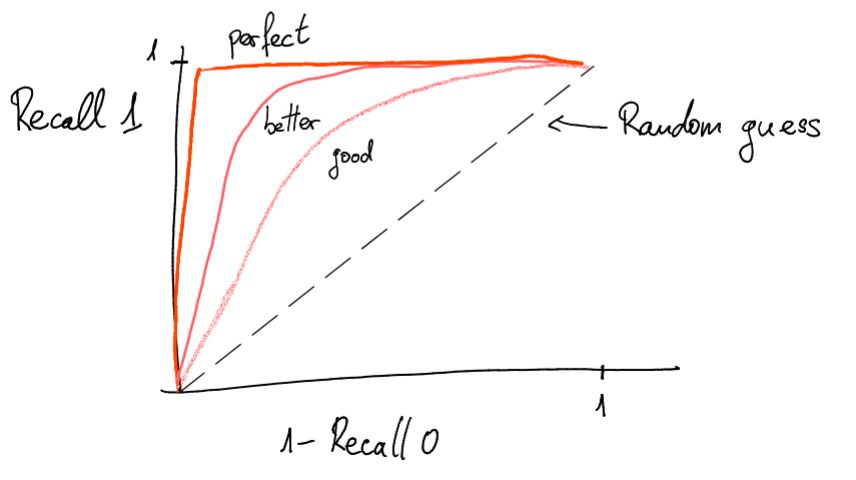
\includegraphics[width = .8\linewidth]{images/ROC}
\caption{ROC curve for a binary classifier. Ideally, the classifier will be as far as possible from the random guess, and maximize the recall in classes 0 and 1 at the same time. }
\label{fig.roc}
\end{figure}

\subsection{Common gradient-descent optimizers -- ADAM}

The ADAM optimizer \cite{kingma2017adam} is one of the most common gradient descent optimizers, widely used in machine learning and neural networks. In words of the authors 
\begin{quote}
The method is straightforward to implement, is computationally efficient,
has little memory requirements, is invariant to diagonal rescaling of the gradients,
and is well suited for problems that are large in terms of data and/or parameters.
The method is also appropriate for non-stationary objectives and problems with
very noisy and/or sparse gradients.
\end{quote}

\begin{figure}
\centering
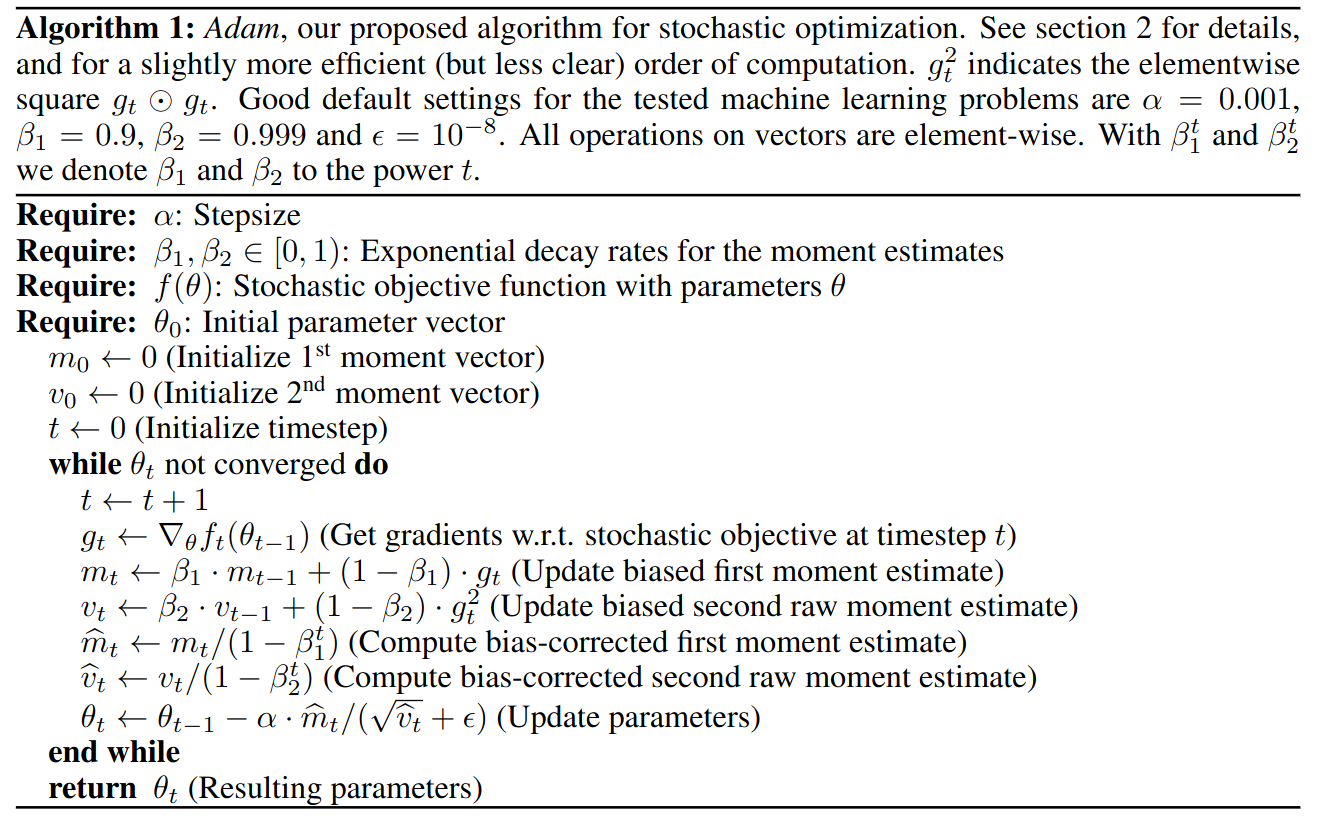
\includegraphics[width = \linewidth]{images/adam}
\end{figure}

The ADAM optimizer is based on averages of gradients, given to the first and second order, by $m_t$ and $v_t$ respectively in the code. During the first timesteps, the algorithm provides large variabilty in these averages, while as the iteration number grows they converge to a stationary point. This is achieved by controlling the hyperparameters $\alpha, \beta_1, \beta_2$, which make the influence of each new step decay in each new iterations. 

\chapter{Introduction to TensorFlow}\label{sec.tensorflow}

As we have seen in previous chapters, it is possible to create NNs, SVMs and also other models for machine learning. However, the current extensive usage of machine learning is only possible due to the existence of dedicated hardware and software packages with specific optimization. Most of these packages are highly developed packages with pre-defined computations and automatic pipelines that allow researchers and data scientists to create machine learning models with small effort and high efficiency, in a plug-and-play strategy. All within a matter of minutes. In this chapter, we will review one of these tools: TensorFlow. 

TensorFlow is a machine learning pipeline developed by Google. It machinery is very easy to understand and scalable. It consists of \textit{layers}, that can be combined to build mainly NNs with a flexible architecture. The only requirement is to make the relative sizes of consecutive layers match, to effectively pass the information forward to the NN. After the architecture is designed, all the backpropagation accesory elements needed to conduct the learning of some unknown data is pre-implemented in the software, and it is possible to perform the entire learning process with a few lines of code. 

See for instance the code below.
\vskip5mm

\begin{boxedverbatim}
import tensorflow as tf

mnist = tf.keras.datasets.mnist

(x_train, y_train), (x_test, y_test) = mnist.load_data()
x_train, x_test = x_train / 255.0, x_test / 255.0

model = tf.keras.models.Sequential([
  tf.keras.layers.Flatten(input_shape=(28, 28)),
  tf.keras.layers.Dense(128, activation='relu'),
  tf.keras.layers.Dropout(0.2),
  tf.keras.layers.Dense(10, activation='softmax')
])

model.compile(optimizer='adam',
              loss='sparse_categorical_crossentropy',
              metrics=['accuracy'])

model.fit(x_train, y_train, epochs=5)

model.evaluate(x_test,  y_test, verbose=2)

\end{boxedverbatim}
\vskip5mm

This code performs the following steps
\begin{enumerate}
\item Load the TensorFlow package
\item Load the dataset of interest. This step is here for demonstration purposes, since the MNIST dataset is a very common dataset to test machine learning models. The MNIST dataset is composed by squared images (28 x 28 in the format of TensorFlow) of handwritten digits. The goal of the learning process is to recognize the number written in each of the images. 
\item Preprocess the data.
\item Generate a model composed by the following layers 
\begin{enumerate}
\item A \textit{flatten} layer, to transform a square image into a 1-dimensional array
\item A dense fully connected layer, as in \Cref{sec.neural-networks}
\item A dropout layer with probability 0.2 to drop (transform to zero)
\item A second fully connecter layer with output 10, which is the number of classes required.
\end{enumerate}
\item Compiling the model, to enhance performance for computation. This step has the information of which optimizer to use, which loss to use for training, and how to benchmark the accuracy for the trained model. 
\item Fit, or train, the model with respect a training data. 
\item Evaluate the model in the training data. 
\end{enumerate}
The official guide of TensorFlow confirms that this model trains within a few seconds, and achieves accuracies of classification of nearly $\sim 98 \%$. 

The performance of these models depend mainly on how the compilation process works. At this step, TensorFlow is capable of very effectively dealing with hardware acceleration, for instance using GPUs or parallelism. There exist exhaustive resources to optimize code to be used in TensorFlow (or similar) packages, that can boost the data analysis capabilities of almost any kind of data. 

TensorFlow is highly optimized to perform the tasks it was designed for. However, the only flexibility one can use is the one that has been foreseen. Creating customized models is possible, but it requires deeper knowledge of the internal machinery to ensure compatibility of all the required elements. 

For the next sessions, it is recommendable to refer to the Notebooks. 

\section{Neural networks with TensorFlow}

TensorFlow does not add anything fundamentally new on NNs to be added to the content given in the previous chapter. However, TensorFlow is highly optimized to run large NNs on high-dimensional data and perform classification tasks in a matter of seconds. For instance, consider the MNIST dataset, that is handwritten numbers as in \Cref{fig.mnist}. A code of the form
\vskip5mm

\begin{boxedverbatim}
import tensorflow as tf
((X_train, y_train), (X_test, y_test)) = mnist.load_data()

# We create now the model through the application of several layers. 

model = tf.keras.models.Sequential([
  tf.keras.layers.InputLayer(shape=(28, 28)) , 
  tf.keras.layers.Flatten(input_shape=(28, 28)), # Transformation of squared images to 1-dimensional arrays
  tf.keras.layers.Dense(128, activation='relu'), # fully connected layer, with output 128
  tf.keras.layers.Dense(10)                      # Second layer, with output 10, and final layer
])

model.compile(
    optimizer=tf.keras.optimizers.Adam(0.001), # Optimizer, can be changed
    loss=tf.keras.losses.SparseCategoricalCrossentropy(from_logits=True), # Loss function, can be changed
    metrics=[tf.keras.metrics.SparseCategoricalAccuracy()], # Metrics, to check the performance
)

model.fit(
    X_train, y_train, epochs = 10
) # In each epoch, the training data is shuffled to improve learning


model.compile(
    optimizer=tf.keras.optimizers.Adam(0.001), # Optimizer, can be changed
    loss=tf.keras.losses.SparseCategoricalCrossentropy(from_logits=True), # Loss function, can be changed
    metrics=[tf.keras.metrics.SparseCategoricalAccuracy()], # Metrics, to check the performance
)

model.fit(
    X_train, y_train, epochs = 10
) # In each epoch, the training data is shuffled to improve learning

test_loss, test_acc = model.evaluate(X_test, y_test, verbose=2)

print('\nTest accuracy:', test_acc)

y_pred = np.argmax(model.predict(X_test), axis = 1)
\end{boxedverbatim}
\vskip5mm

is capable of returning a prediction accuracy of $97,34\%$ within a training time of 30 seconds in a laptop. The prediction can be seen in \Cref{fig.mnist}. 

\begin{figure}\centering
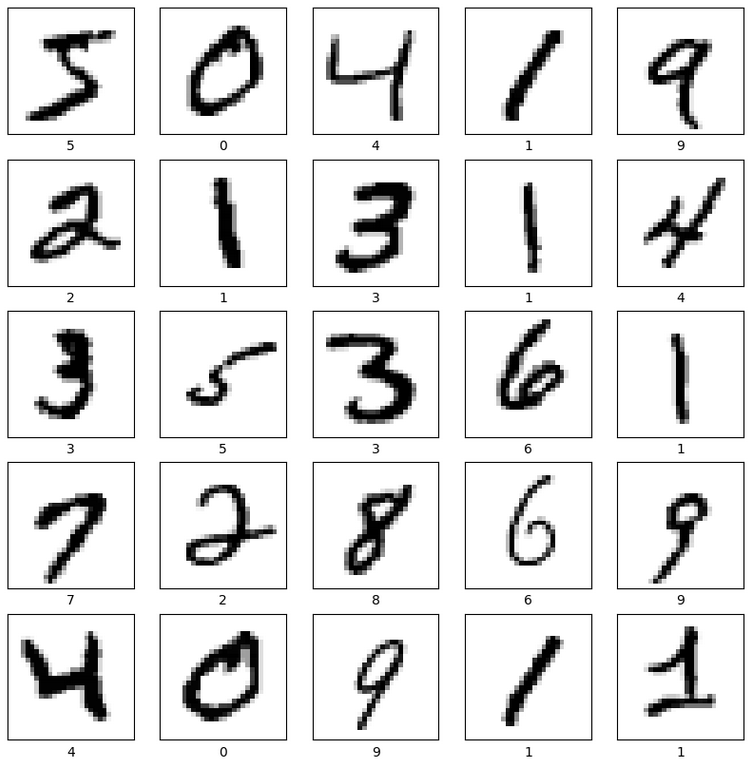
\includegraphics[width = .475\linewidth]{images/mnist}
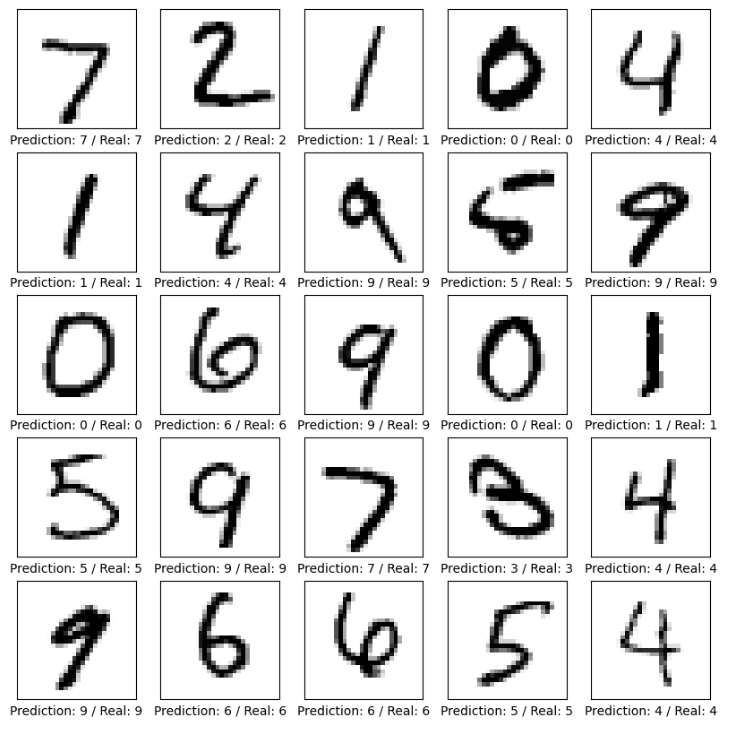
\includegraphics[width = .485\linewidth]{images/prediction-mnist}
\caption{The MNIST dataset of handwritten digits (left) and its predicted classification using a simple \texttt{TensorFlow} neural network.}
\label{fig.mnist}
\end{figure}

\subsection{Fashion MNIST dataset}

We can use TensorFlow to classify more complex datasets, in particular one of images obtained from a catalogue of clothes. This dataset, the Fashion MNIST, as well as the digits MNIST, are common testbeds for machine learning algorithms. Performing a similar neural network from the one obtained in the previous example, we can see the results in \Cref{fig.fashion-mnist}. 

\begin{figure}\centering
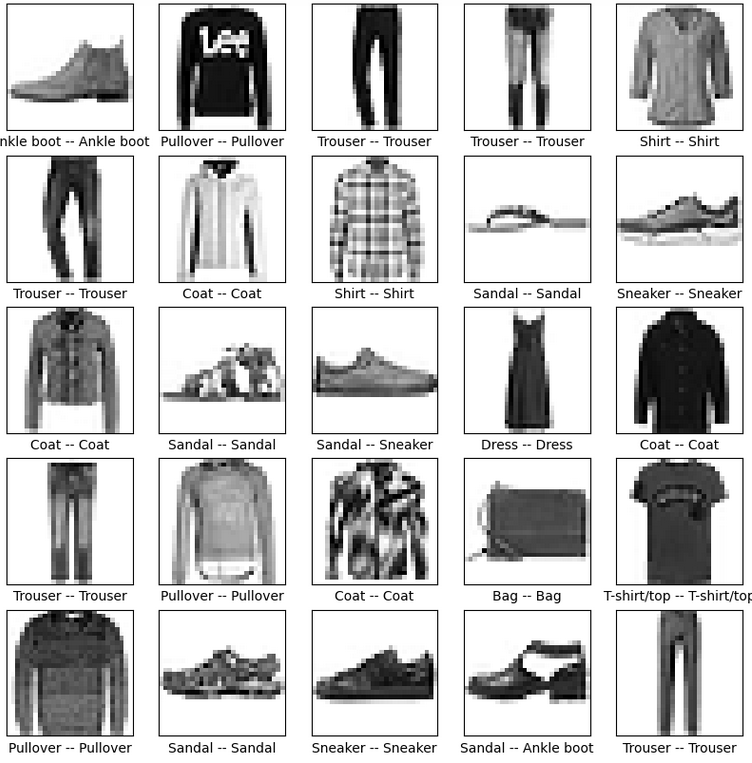
\includegraphics[width = .7\linewidth]{images/fashion-mnist}
\caption{The prediction of a \texttt{TensorFlow} simple neural network on the Fashion MNIST dataset of clothes images.}
\label{fig.fashion-mnist}
\end{figure}

For this classification task, we have added a convolutional layer, which is designed to work well for image classification. In this case, the training is longer, of ca. 5 minutes in a laptop. 

\vskip5mm

\begin{boxedverbatim}
import tensorflow as tf
((X_train, y_train), (X_test, y_test)) = fashion_mnist.load_data()

# We create now the model through the application of several layers. 
# IN this example we use a convolutional neural networks, that we have mentioned it is ideal for image processing

# Question: Do we need it?

model = tf.keras.models.Sequential([
  tf.keras.layers.InputLayer(shape=(28, 28, 1)), 
  tf.keras.layers.Conv2D(10, 2, input_shape=(28, 28, 1)), # Convolutional layer of squared images
  tf.keras.layers.Flatten(input_shape=(10, 10)), 
  tf.keras.layers.Dense(128, activation='relu'), # fully connected layer, with output 128
  tf.keras.layers.Dense(10)                      # Second layer, with output 10, and final layer
])

model.compile(
    optimizer=tf.keras.optimizers.Adam(0.001), # Optimizer, can be changed
    loss=tf.keras.losses.SparseCategoricalCrossentropy(from_logits=True), # Loss function, can be changed
    metrics=[tf.keras.metrics.SparseCategoricalAccuracy()], # Metrics, to check the performance
)

model.fit(
    X_train, y_train, epochs = 10
) # In each epoch, the training data is shuffled to improve learning


\end{boxedverbatim}
\vskip5mm

\subsection{Classifying the Ising model}\label{sec.ising}

In the final example for neural networks, we will use TensorFlow to classify data from an Ising model, a common example in statistical Physics. The Ising model is defined by a Hamiltonian of the form
\begin{equation}
H = -\sum_{i, j} s_i s_j, 
\end{equation}
with $s_i, s_j$ being spins up and down, organized over a square lattice. The goal of the Ising model is to obtain the state at which the model ended, as a function of the temperature. We can identify two main cases in the Ising model, mainly the ferromagnetic and antiferromagnetic phases, or ordered and disordered. In a nutshell, for low temperatures, the system will naturally fall into a low-energy state, that is $s_i = s_j$. On the other hand, for high temperatures, the thermal excitations allow for disordered phases. The phase transition happens at $T = 2.269 K$. See \Cref{fig.phases} for a graphical example of both phases. 

\begin{figure}\centering
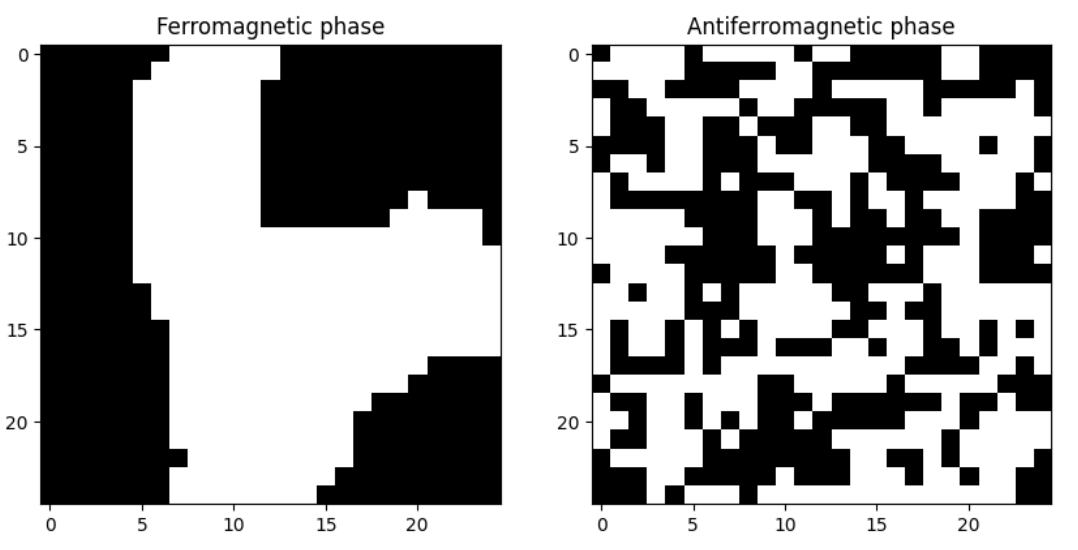
\includegraphics[width = .8\linewidth]{images/ising}
\caption{Two Ising phases: ferromagnetic or ordered (left) and antiferromagnetic or disordered (right). }
\end{figure}

We can use tensorflow to classify data from both phases using neural networks and the states (or images) as data. A code of the following form suffices to achieve accuracies over $95\%$.



\vskip5mm

\begin{boxedverbatim}
import tensorflow as tf
from tensorflow import keras
from keras.models import Sequential
from keras.layers import Dense, Activation
from keras.regularizers import l2

# Initialize model
model = Sequential()

# Add hidden layer with 32 units and rlu activation. Add output layer with sigmoid activation.
model.add(Dense(25, activation='relu', kernel_regularizer=l2(0.1), input_dim=25**2))
model.add(Dense(15, activation='relu', kernel_regularizer=l2(0.1)))
model.add(Dense(1, activation='sigmoid'))

# Compile model
model.compile(optimizer='Adam', loss='binary_crossentropy', metrics=['accuracy'])

# Fit model
model.fit(X, y, epochs=40, verbose=0)

# Add training and test errors to lists
train_errors = model.evaluate(X,y,verbose=0)[1]
test_errors = model.evaluate(X_test,y_test,verbose=0)[1] 
\end{boxedverbatim}
\vskip5mm

\section{Generative modeling with TensorFlow}\label{sec.generative-tensorflow}

Generative modelling is more complicated than just classification. In this example we will use adversarial training to construct a generative algorithm. 

Adversarial training is composed by two elements: the generator and the discriminator. The generator is the neural networks from which new samples will be taken. Alternatively, the discriminator is a trained model capable of distinguishing whether a given data is taken from the dataset or not. This yields two different cost functions,
\begin{align}
\mathcal L_{\rm Gen} & = -\frac{1}{\vert \mathcal T_{\rm Gen} \vert}\sum_{x \in \mathcal T_{\rm gen}} D(x)\\
\mathcal L_{\rm Disc} & = \frac{1}{\vert \mathcal T_{\rm Gen} \vert}\sum_{x \in \mathcal T_{\rm gen}} D(x) - \frac{1}{\vert \mathcal T_{\rm Real} \vert}\sum_{x \in \mathcal T_{\rm Real}} D(x)
\end{align}
which compete. In our case, use the cross-entropy between two probability distributions, but any other can be in principle used. Since both the generator and the discriminator are neural networks, one can use the backpropagation trick to compute gradients and update the network, allowing for an efficient training process. From this point, it is possible to choose an optimizer that completes the work for us. The optimizer just applies gradient-descent-like algorithms. 


 [TO BE COMPLETED]


\chapter{Quantum Machine Learning}

Quantum machine learning (QML) is the discipline that combines quantum computing with machine learning to leverage quantum processing capabilities. 

There exist several relevant concepts that distinguish classical and quantum types of machine learning, and that also distinguish QML from pure quantum computing. 

\paragraph{Quantum computing in a nutshell --} Quantum computing is a new paradigm for computation stemming from translating bits, that is units of information with the states $0 / 1$ into qubits, quantum units of information that can take any superposition 
\begin{equation}
\ket q = \alpha\ket 0 + \beta\ket 1.
\end{equation}
A $n$-qubit quantum state, in full generality, is written as
\begin{equation}
\ket\psi = \sum_{i = 0}^{2^n - 1} \alpha_i \ket i, 
\end{equation}
under the constraint that $\braket{\psi}{\psi} = 1$. 

In classical computing, available classical operations are those functions transforming bitstrings into bitstrings. All logical operations can be performed by combining FANOUT (copies) and NAND operations, that is 
\begin{align}
\operatorname{NAND}(0, 0) & = 1 \\
\operatorname{NAND}(0, 1) & = 1 \\
\operatorname{NAND}(1, 0) & = 1 \\
\operatorname{NAND}(1, 1) & = 0 .
\end{align}

In the case of quantum computing, the available logical operations are unitary gates $U \in \mathcal SU(2^n)$, allowing for a much larger variety of operations. For instance, a single-qubit quantum gate is any operation of the form
\begin{equation}
U(\theta, \phi, \lambda) = \begin{pmatrix}
\cos(\theta) & -\sin(\theta) e^{i\phi} \\
\sin(\theta) e^{i\lambda} & \cos(\theta) e^{i\phi} e^{i\lambda}
\end{pmatrix}
\end{equation}

This change of paradigm allows quantum computers to perform operations that cannot be efficiently computed with classical resources. 

\paragraph{Efficiency of computations --} A key concept is complexity theory is that of efficiency of computations, that is, what is the computational cost of running a given algorithm, in terms of operations. The predominant argument is scaling, that is, what is the functional form that dominates the effort, with respect to the size of the problem $n$. For example, if an algorithm runs in time
\begin{equation}
T(n) = 56 n^4 + 4n^2 \log n + n \log n + n^{-2}, 
\end{equation}
we say that 
\begin{equation}
T(n) \in \mathcal O(n^4) = \mathcal O({\rm poly}(n)).
\end{equation}
By convention, an algorithm is called efficient if it runs in $\mathcal O({\rm poly}(n))$ time steps and needs a memory storage of the same size. On the other hand, if the cost exceeds polynomial scaling (even by a bit), the algorithm is considered as inefficient. In the end, the relevant 

Notice that this convention might be unpractical in realistic settings. Consider for example two algorithms, with running times
\begin{align}
T_1(n) & \in \mathcal O(n^{10}) \\
T_2(n) & \in \mathcal O(n^{\log n}).
\end{align}
The scaling of $T_2(n)$ is faster than that of $T_1(n)$, hence it is in the long run desirable to use $T_1(n)$. However, for moderate problem sizes, it is reasonable that a worst scaling is preferrable for practical reason. The same argument holds for prefactors, which are not captured by big-O scalings. 

\paragraph{Simulability --} Simulability is a concept that relates different computational paradigms. If two computing paradigms are universal, for example classical and quantum, then both can perform any arbitrary operation. However, it might be the case that one of the paradigm achieves this operation using less \textit{basic} operations than the other. Depending on how much the difference is, then it will be possible to simulate one system with the other. 

In particular, we mention that a quantum computation is simulable with a classical computer if $T_C / T_Q \in \mathcal O({\rm poly} (n))$, where $n$ is the number of qubits. These considerations might also depend on the error of the simulation process, thus allowing not for exact computations, but approximate results. 

Notice that in principle it should be easy to find quantum computations that are not simulable. Storing a quantum state in a classical computer requires $\mathcal O(2^n)$ memory, and any operation will demand similar times to be executed. Assume now that we want to compute a particular property of the quantum state, such as an expectation value or the overlap with respect to a given state. Since this is a limited information, there exist many cases in which partial descriptions of quantum states suffice to extract the information of interest. Examples of this kind are tensor networks \cite{orus2014practical} or stabilizer states \cite{gottesman1998heisenberg}. 

Hence, it is in general not trivial to assess whether a quantum computation is classically simulable or not, or for which interesting problems there exist classical approaches. The class of computations that are quantumly easy but classically hard are called BQP (Bounded Quantum Polynomial) operations. The most celebrated example of a BQP problem is Shor's algorithm \cite{shor1997polynomialtime}, which is capable of solving the problem of factoring an integer number $N = pq$, for $p$ and $q$ primes, and the discrete logarithm problem (DLP), that is, given $x$, finding $y$ such that $x = g^y \mod N$.

\paragraph{Dequantization --} Dequantization is the process of transforming a QML algorithm into a classical algorithm, i. e. to be ran in a \textit{classical} computer, that performs the same or similar task. The classical version of the algorithm does not need to be similar or inspired by the quantum, it only needs to perform the same task. 

Dequantization is conceptually related but different from simulability of quantum computing. For a quantum algorithm to be simulable, we need a classical computer capable of performing exactly the same operation. However, for a quantum algorithm to be dequantizable, we just need a classical algorithm that performs the same task, maybe through different methods. Examples of this concept will appear in \Cref{sec.re-uploading}.

\paragraph{The power of (quantum) data --}

This chapter will cover some examples and basic concdpts of quantum machine learning, together with examples of the problems in a computer. I will use {\tt QIBO} for it.  

\section{Kernels in quantum machine learning}

Kernels are most direct example to apply machine learning with quantum computers. For the kernels, consider a data-dependent unitary operation $V(x)$ capable of applying a map to an initial state, that is
\begin{equation}
\ket{\psi(x)} = V(x) \ket 0.
\end{equation}
Computing the kernel of this feature map is easy, by just computing
\begin{equation}
k(x_i, x_j) = \vert \braket{\phi(x_i)}{\psi(x_j)} \vert^2 = \vert \bra 0 V^\dagger (x_i) V(x_j) \ket 0 \vert^2.
\end{equation}
From this point on, applying QML is equivalent to using a SVM to solve a learning problem, with the modification that the new kernel cannot be (in principle) computed using classical resources. 

For an illustrative example, consider this example in \Cref{fig.havlicek-kernel} \cite{havlicek2019supervised}. The depicted feature map transforms $x \in \mathbb R^2$ into a real number $y \in [-1, 1]$. The goal is to find the sign of $y$. By applying the kernel trick from SVM with this kernel, we can classify this data. 
Generating this data using classical resources is hard because the considered circuit has properties to avoid classical simulability\footnote{Upon scaling in qubits and specific circuit architectures}. Notice however that the role of the quantum computer is not to learn the classification, but to transport the data into a linear subspace where classification is doable with linear separations. 

\begin{figure}
\centering
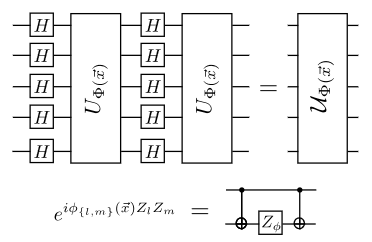
\includegraphics[height = .3\linewidth]{images/havlicek-kernel1}
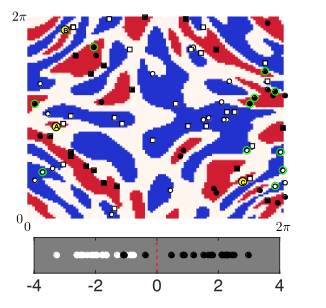
\includegraphics[height = .3\linewidth]{images/havlicek_data}
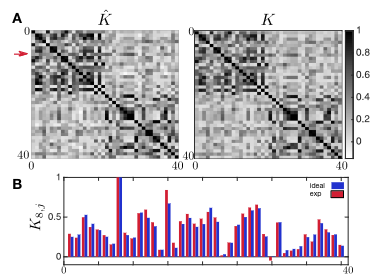
\includegraphics[width = .6\linewidth]{images/havlicek-kernel2}
\caption{Classification problem using a quantum kernel, as seen in \cite{havlicek2019supervised}. The dataset is generated from the quantum kernel, making it a perfect candidate for using quantum classifiers as the optimal classification tool. }
\label{fig.havlicek-kernel}
\end{figure}

\begin{figure}
\centering
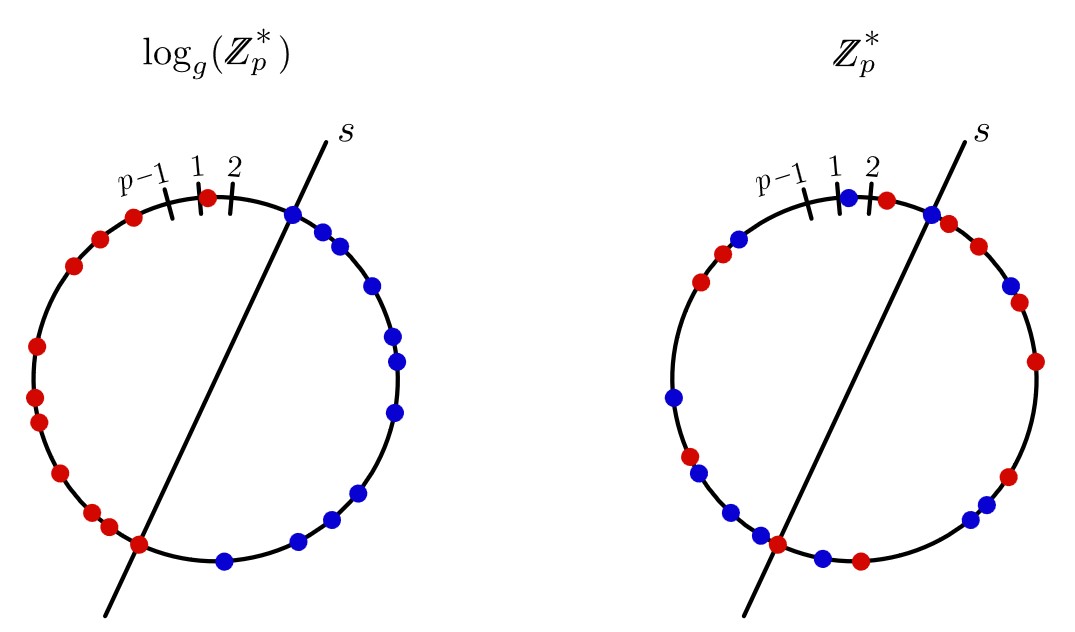
\includegraphics[width=.6\linewidth]{images/DLP}
\caption{Representation of the DLP kernel, used to solve a classification task with provable quantum advantage. }
\label{fig.dlp}
\end{figure}

Kernels in QML may suffer from the \textit{curse of dimensionality}. The Hilbert space in which quantum states are embedded is exponentially large. If two states $\ket\psi, \ket\phi$ are chosen at random, their relative overlap will be $\sim e^{-n}$ with high probability \cite{thanasilp2024exponential}. This means that any kernel matrix used with this kernel will be close to the identity, meaning all points have almost zero overlap with all other points, irrespective of their classes. That being the case, the QML algorithm is effectively capable of learning the training data, but performs randomly on unseen data.  

\subsection{Discrete Logarithm Problem and quantum advantage}\label{sec.dlp}

The existence of BQP problems can be used to prove that there exist learning problems that cannot be solved with a classical computer \cite{liu2021rigorous}. 

Consider the following problem. Let $\mathbb Z_p^*$ be the data space, that is the cyclic group $Z_p^* = \{0, 1,2,\ldots p-1 \}$. Let $n = \lceil  \log_2 p \rceil$. For any $s \in \mathbb Z_p^*$ define the mapping
\begin{equation}
f_s(x) = \left\{ 
\begin{matrix}
1 & \log_g x \in [s, s + (p - 3) / 2] \\
-1 & {\rm else}
\end{matrix}
\right.
\end{equation}
This mapping divides the data space into two classes of the same size. 

Based on assumptions of the DLP problem, one can make use of the following feature map to use a SVM that is capable of solving the problem. The kernel is given by
\begin{equation}
\ket{\psi_{y, k}} = \frac{1}{\sqrt{2^k}} \sum_{i \in \{ 0, 1\}^k } \ket{y g^{i}}, 
\end{equation}
for a $k$ to be specified later. The kernel is given by
\begin{equation}
C(y_i, y_j) = \vert \braket{\psi_{y_i, k}}{\psi_{y_j, k}}\vert^2.
\end{equation}
Assuming that $y = g^x$, the states previously given can be understood as interval states, that is, states that span all states in the interval $[x, x+1, \ldots, x + 2^k - 1]$. The kernel is thus equivalent to computing intersection of the corresponding intervals. 

The DLP mapping admits an interpretation in terms of scrambling. The modular exponentiation transforms $y = g^x$, which is nothing but a hard-to-describe permutation. The inversion is hard to compute classically. By creating the previously defined kernels, we are covering sufficiently many cases of the DLP to ensure that, if two data points correspond to the same class, then the kernel will be sufficiently far from $0$, hence a margin classification is possible. 


The key element of this problem is that the kernel is efficient to apply only for quantum computers. For one particular element, computing the modular exponentiation is easy. The difficulty arises when exponentially many of these elements are considered simultaneously, as given in this case. Shor's algorithm \cite{shor1997polynomialtime} shows efficiency for this kernels. In particular, it is proven that if this problem is solvable with a classical machine, then there exists a classical algorithm to solve the DLP.  

\section{Variational quantum machine learning}\label{sec.variational}

Variational quantum computing witnessed a large growth in the last decade, from its inception \cite{peruzzo2014variational}. Variational methods consist in applying parameter-dependent quantum circuits $U(\theta)$. These circuits can help with solving current hardware limitations in state-of-the art prototypes, including but not limited to available number of qubits, tolerance to error or number of operations. For comprehensive reviews, see \cite{bharti2022noisy, cerezo2021variational}

The functioning principle of a variational quantum algorithm is as follows. An ansatz of the form $\ket{\psi(\theta)} = U(\theta)\ket 0$ is used to generate a quantum state encoding the solution of a problem of interest. The problem itself is encoded in a Hamiltonian $H$. Solving the problem of interest becomes equivalent to finding the ground state of this Hamiltonian, and the optimal parameters are given by
\begin{equation}
\theta^* = \operatorname{argmin}\left( \bra{\psi(\theta)}H\ket{\psi(\theta)}\right).
\end{equation}
In general, solving this problem is hard and intractable, belonging to the class QMA \cite{kempe2005complexity}.

\subsection{Variational kernel-based quantum machine learning}

There exists an alternative interpretation of kernels for QML. The aforementioned feature map can be understood is only a manner to input data into a quantum circuit. Then, one can use an optimized measurement strategy to perform classification. This strategy, which has been extensively used in research, plays the role of solving the optimization problem in a kernel-tricked SVM. 



Consider the kernel problem previously mentioned. The feature map can be followed by a tunable quantum operation, and then a fixed observable. In the Heisenberg picture, optimizing the quantum circuit is equivalent to finding the optimal measurement \cite{helstrom1976quantum}. By the representer theorem, one can rewrite this problem in terms of kernels. This means that the feature map is crucial for the performance of the classification, since it upper bounds the possible distinction between classes even of the optimal measurement strategy. 

\begin{figure}
\centering
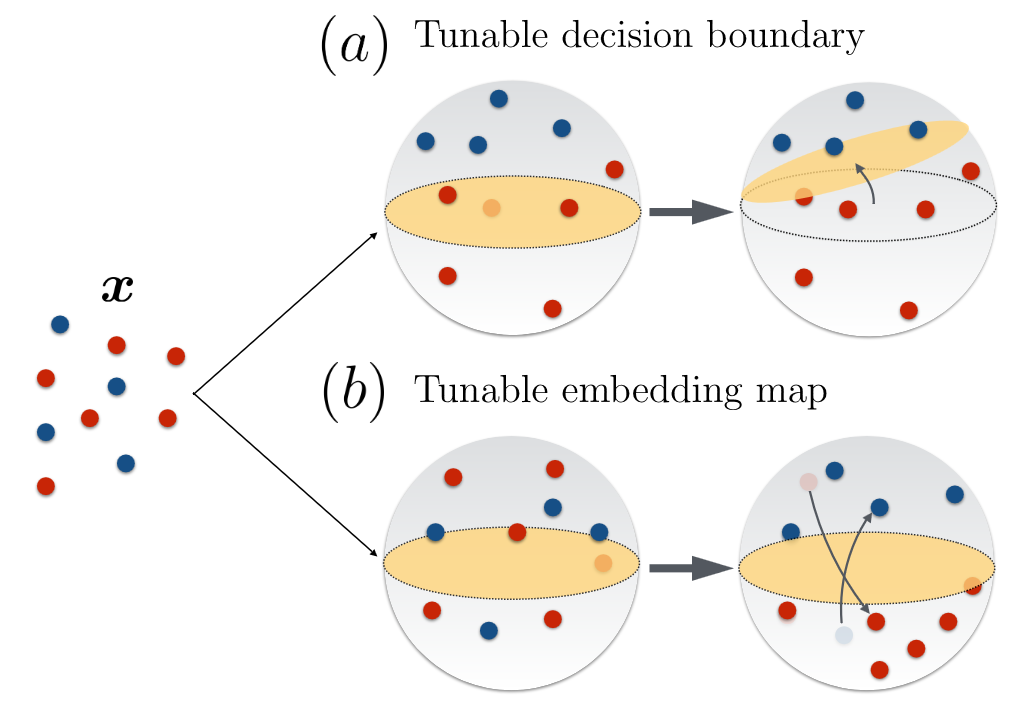
\includegraphics[width = .6\linewidth]{images/berta}
\caption{}
\label{fig.berta}
\end{figure}

\subsection{Data re-uploading for quantum machine learning}\label{sec.re-uploading}

One can consider the option of constructing a tunable kernel, so that the feature map is capable of effectively \textit{learning} the data and adapt the transformation from the data to the feature space to the target function to be learnt. A method to achieve this goal is the so-called \textit{re-uploading} scheme. This method is characterized by creating feature maps as
\begin{equation}
U(x, \theta) = \prod_{i = 1} V(x) W(\theta_i). 
\end{equation}
It is possible to show that the function generated by
\begin{equation}
h_\theta(x) \equiv \bra 0 U^\dagger(x, \theta) H U(x, \theta) \ket 0 
\end{equation}
satisfy universality theorems in a similar way as in \Cref{sec.universality-nn}, even for single qubit quantum circuits. This provides a \textit{theoretical} capability of these parameter-dependent kernels to solve any kind of learning problems. The interpretation of re-uploading kernels is available in \Cref{fig.berta}. It has been recently shown that re-uploading schemes, used for quantum data, can also provide universality in the achieved functions \cite{perez-salinas2024universal}, with $\log d$ qubits, being $d$ the dimensionality of the data. 

\begin{figure}\centering
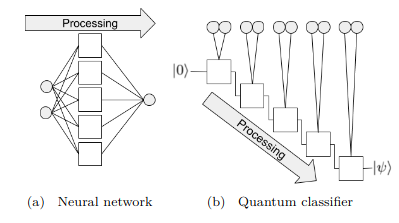
\includegraphics[width = .7\linewidth]{images/reuploading}
\caption{Scheme for a re-uploading strategy in a quantum computer, and comparison to a single-layer neural network. In both cases, data is uploaded several times into the pipeline. }
\label{fig.reuploading}
\end{figure}

\subsection{Variational algorithms lack biases}

An important issue of variational quantum algorithms is that of \textit{barren plateaus} (BP) \cite{mcclean2018barren, larocca2022diagnosing}. BPs are the phenomenon of exponential concentration in large-dimensional spaces. It has been repeatedly observed that variational ansatzes for general purpose exhibit poor performances on almost any dataset (for large number of qubits). The reason is that variational ansatzes evely explore the Hilbert space. The outcome states are similar to random states, which unavoidably follow exponential concentrations in any property to be computed. 

In particular, BPs are defined in the literature for fixed-data (or data-less) problems as
\begin{equation}
\operatorname{Var}_{\theta \sim \Theta} \bra 0 U^\dagger(\theta, x) H U(\theta, x) \ket 0, 
\end{equation}
but it is possible to find similar results by considering variances or averages over $x$, kernel considerations or concentrations \cite{thanasilp2024exponential, barthe2024gradients}. 

The take-home message for variational algorithms is to learn from the DLP spirit to solve a problem. We cannot expect QML to work as deep learning, that is, hoping a generic model to learn arbitrary data efficiently. In contrast, we need to rely on specific problems to be solved, and methods that exploit the specific structure of the problem to provide more efficient solutions \cite{aaronson2022how}. Characterizing the gradual transformation from one extreme to the other of the kernel-variational spectrum is still an open question \cite{gil-fuster2024relation}.

\section{Generative modeling for quantum machine learning}

Generative modeling for QML is relevant for its fundamental differences with respect to the previously tracted approaches. As seen in \Cref{sec.generative-modeling}, generative modeling relies on creating samples from a model, with the goal of resembling data taken from an unknown probability distribution. In quantum computing, sampling and computing expectation values are commonly known as strong and weak simulation of quantum computing, implying that sampling is harder (and includes) the computation of expectation values. As a reference, the first demonstrations of quantum advantages rely on sampling problems \cite{arute2019quantum, zhong2020quantum}, and there exist quantum circuits that permit classical simulation to compute expectation values, but not for sampling. [IQP] 

For the reasons stated above, generative modeling must be considered for its possible implications in the findings of quantum advantages. In the following, we will cover the most relevant approaches. 

\subsection{Quantum-circuit Born machines}

A Born is defined as a quantum circuit that creates a quantum state, from which bitstrings are sampled. The probability to sample a bitstring $x$ is given by
\begin{equation}
p_\theta(x) = \vert \bra{x} U(\theta) \ket 0 \vert^2.
\end{equation}
Then, the samples $x$ obtained from the Born machines are compared to the training data, for instance using a Wasserstein distance or a Kullblack-Leibler divergence, to find the configuration of parameters $\theta$ that minimizes these distances. 

If designed variationally, Born machines encode states that resemble samples from the Haar-random distribution of quantum states. This hinders the training of Born machines, for the difficulty of scaping from those configurations, in analogy to the BP phenomenon. 

\subsection{Expectation value samplers}
The expectation value samplers (EVS) are a quantum analogy to classicla models applying arbitrary transformations to random variables, drawn from a simple probability distribution. In these models, we can obtain a set of correlated random variables as
\begin{equation}
x_i = \bra 0 U^\dagger(z, \theta)\hat O_i U(z,\theta)\ket 0, 
\end{equation}
for $z \sim \mathcal N(0, 1)$, for instance. The observables $\hat O_i$ label the different features in the sampled random variable. EVS inherit the properties of the feature map used to transform $z$ into an arbitrary random variable \cite{barthe2024expressivity}. 

\subsection{Quantum Boltzmann machines}
The quantum Boltzmann machine is analogous to the classical one, but the bits have been replaced with qubits. The state of interest is given by the Hamiltonian defining the Boltzmann machine as
\begin{equation}
\rho = \Tr\left( e^{-H}\right)^{-1} e^{-H}. 
\end{equation}
The goal is to optimize $H$, possibly depending on parameters, such that several measurements of the form
\begin{equation}
x_i = \Tr\left( \rho \hat O\right) 
\end{equation}
can be used to solve problems of interest and learning from data. 

Quantum Boltzmann machines are trainable due to sample complexity \cite{coopmans2024sample}, thus they are a promising candidate to build trainable models for quantum machine learning. 


\printbibliography

\end{document}
